%\documentclass[11pt, a4paper]{article} 


%\usepackage{style-3yp}

%\usepackage{geometry} 
%\geometry{%
%a4paper,
%left=20 mm,
%right=20 mm,
%top=20 mm,
%bottom=20 mm
%}
%\usepackage{graphicx} 
%\usepackage{subfigure} 
%\usepackage{float}
%\usepackage{setspace}
%\usepackage[final]{pdfpages}
%\doublespacing
%\begin{document} 

\definecolor{name}{system}{definition}
\definecolor{Gray}{gray}{0.9}
\definecolor{LightCyan}{rgb}{0.88,1,1}
\definecolor{bisque}{rgb}{1.0, 0.89, 0.77}
\definecolor{burntsienna}{rgb}{0.91, 0.45, 0.32}
\section{Hydrogen Production}
\subsection{Introduction} 


Hydrogen gas is required to be fed into the ammonia synthesis process before being converted to energy. The production of hydrogen is currently dominated by the steam reforming of methane gas which depends on the finite fossil fuel resources that also produce greenhouse gases. Water electrolysis combined with renewable energy is sustainable, produces almost zero carbon dioxide and is able to produce hydrogen at a high purity $(>99.9\%)$. Even with these advantages, water electrolysis only represents 4\% of global hydrogen production. This is largely due to high investment cost and energy efficiency problem. There are currently three main types of electrolysis: alkaline electrolysis, polymer electrolyte membrane electrolysis (PEM) and solid oxide electrolysis cell (SOEC). Only the first two types are commercially mature and available. Alkaline electrolysis is chosen because it has the largest power capacity to match the scale of this project. Alkaline electrolysis also has much lower investment cost (at least 10 times smaller)and larger durability compared with PEM. As the maximum power supply (276MW) is far above the power capacity of any commercial electrolysers (typical range is 3 - 6MW), multiple electrolysers are installed in parallel.
The main objective of the design is to increase the system efficiency while maintaining the required hydrogen production rate. The aim of this chapter is to lay a theoretical basis, present a detailed model  and examine the recent trends in alkaline electrolysis technology. 

\subsubsection{Process diagram} 
The process flow diagram in Figure \ref{fig:overview} shows the electrolytic cell and its surrounding facilities, including water treatment, electrolyte recirculation, AC to DC rectifier, output gas treatment, and facilities for temperature and pressure control. The electrolytic cell is the most important component and it also consumes most of the energy supplied. A detailed CAD drawing is shown in next page.

\begin{figure}[H]
\centering
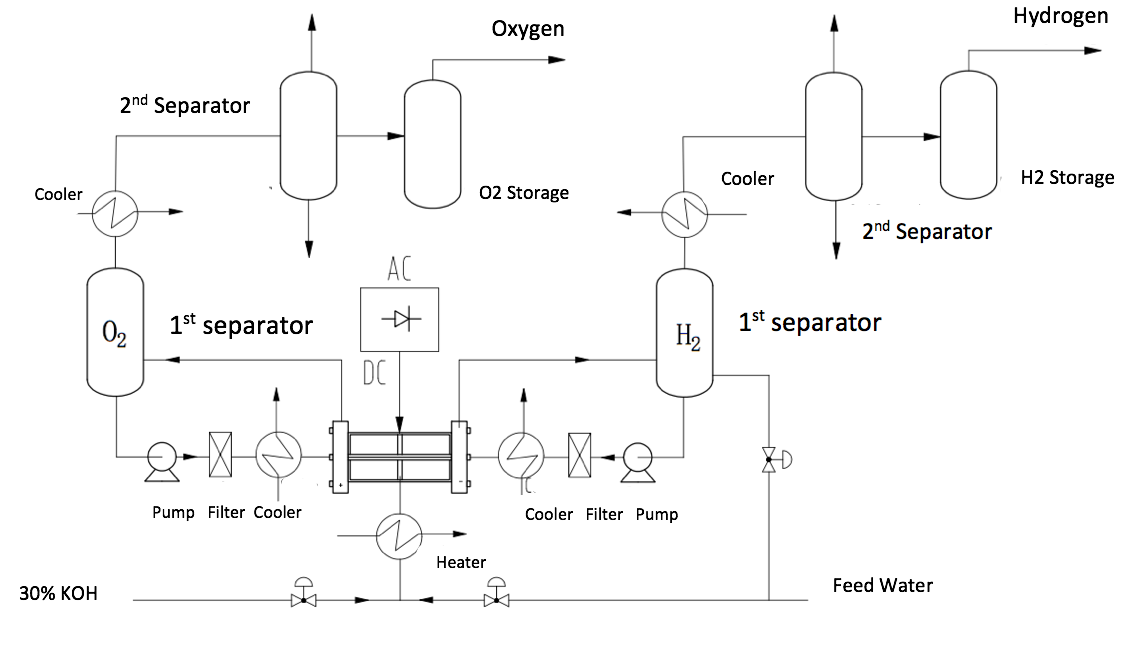
\includegraphics[width= 9 cm] {overview.png} 
\caption{Overview of the system} \label{fig:overview}
\end{figure}  


\begin{figure}[H]
\centering
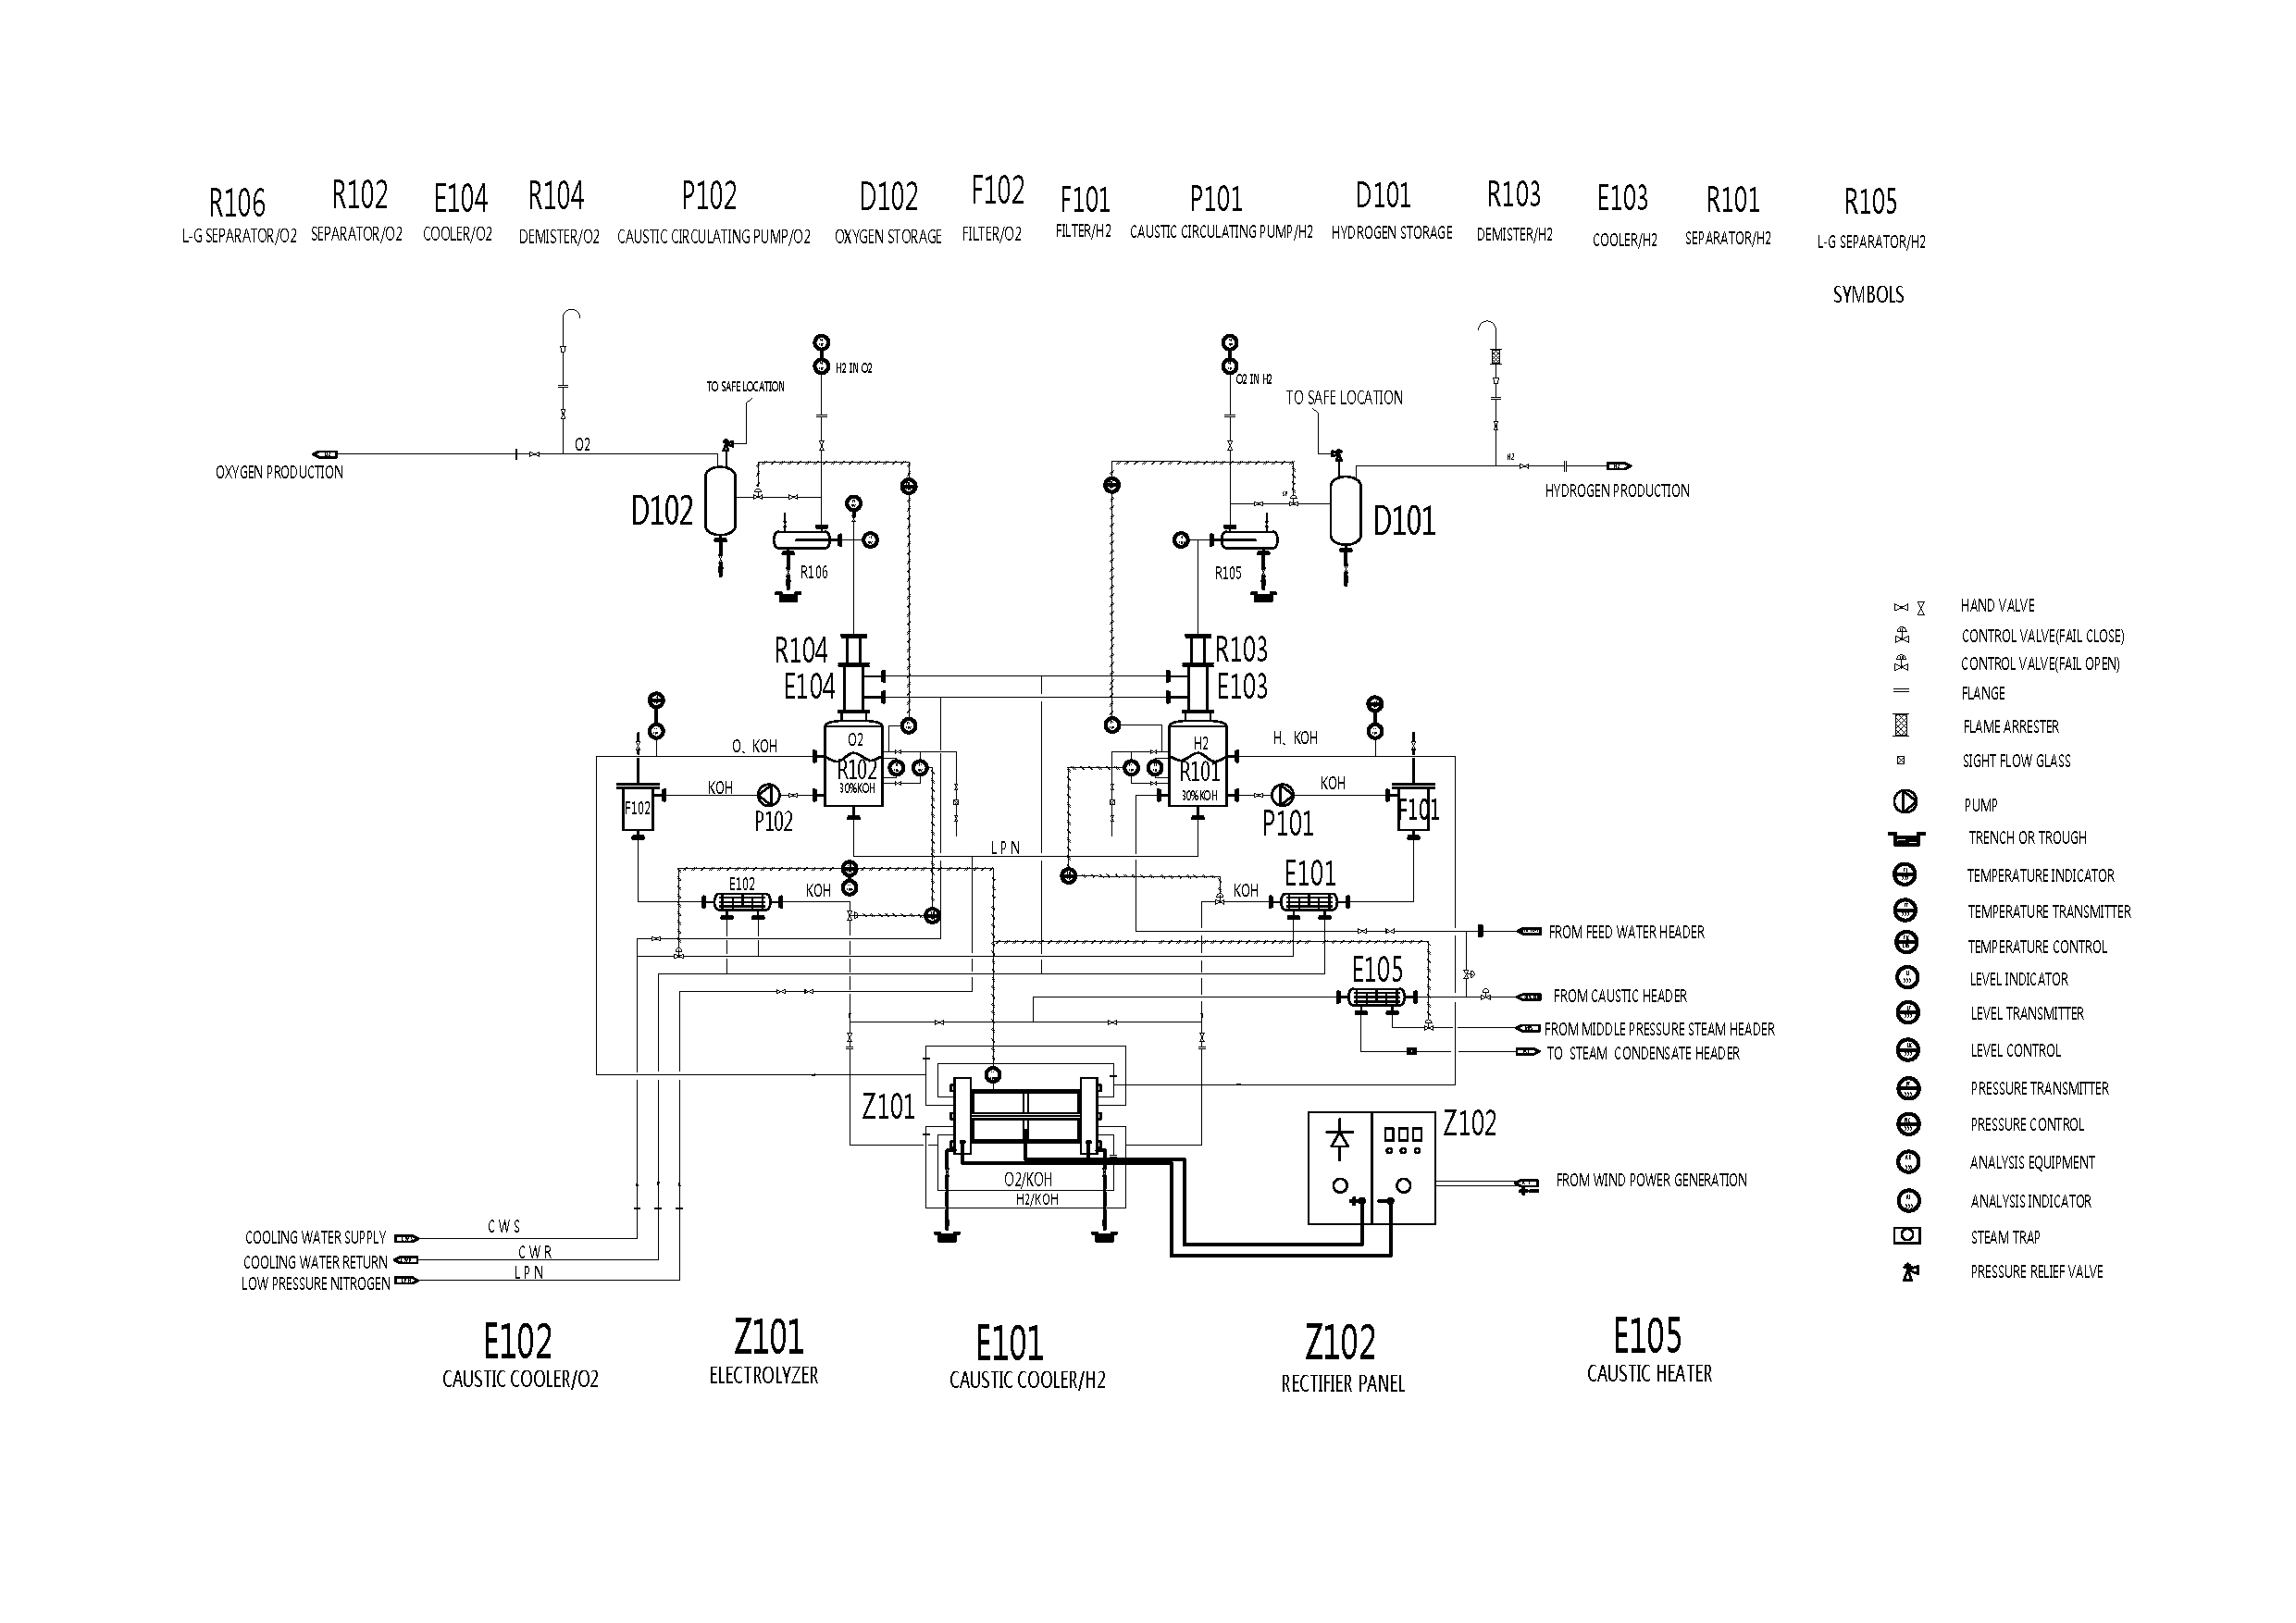
\includegraphics[width= 25 cm, angle=90] {cadcad.pdf}
\end{figure}

%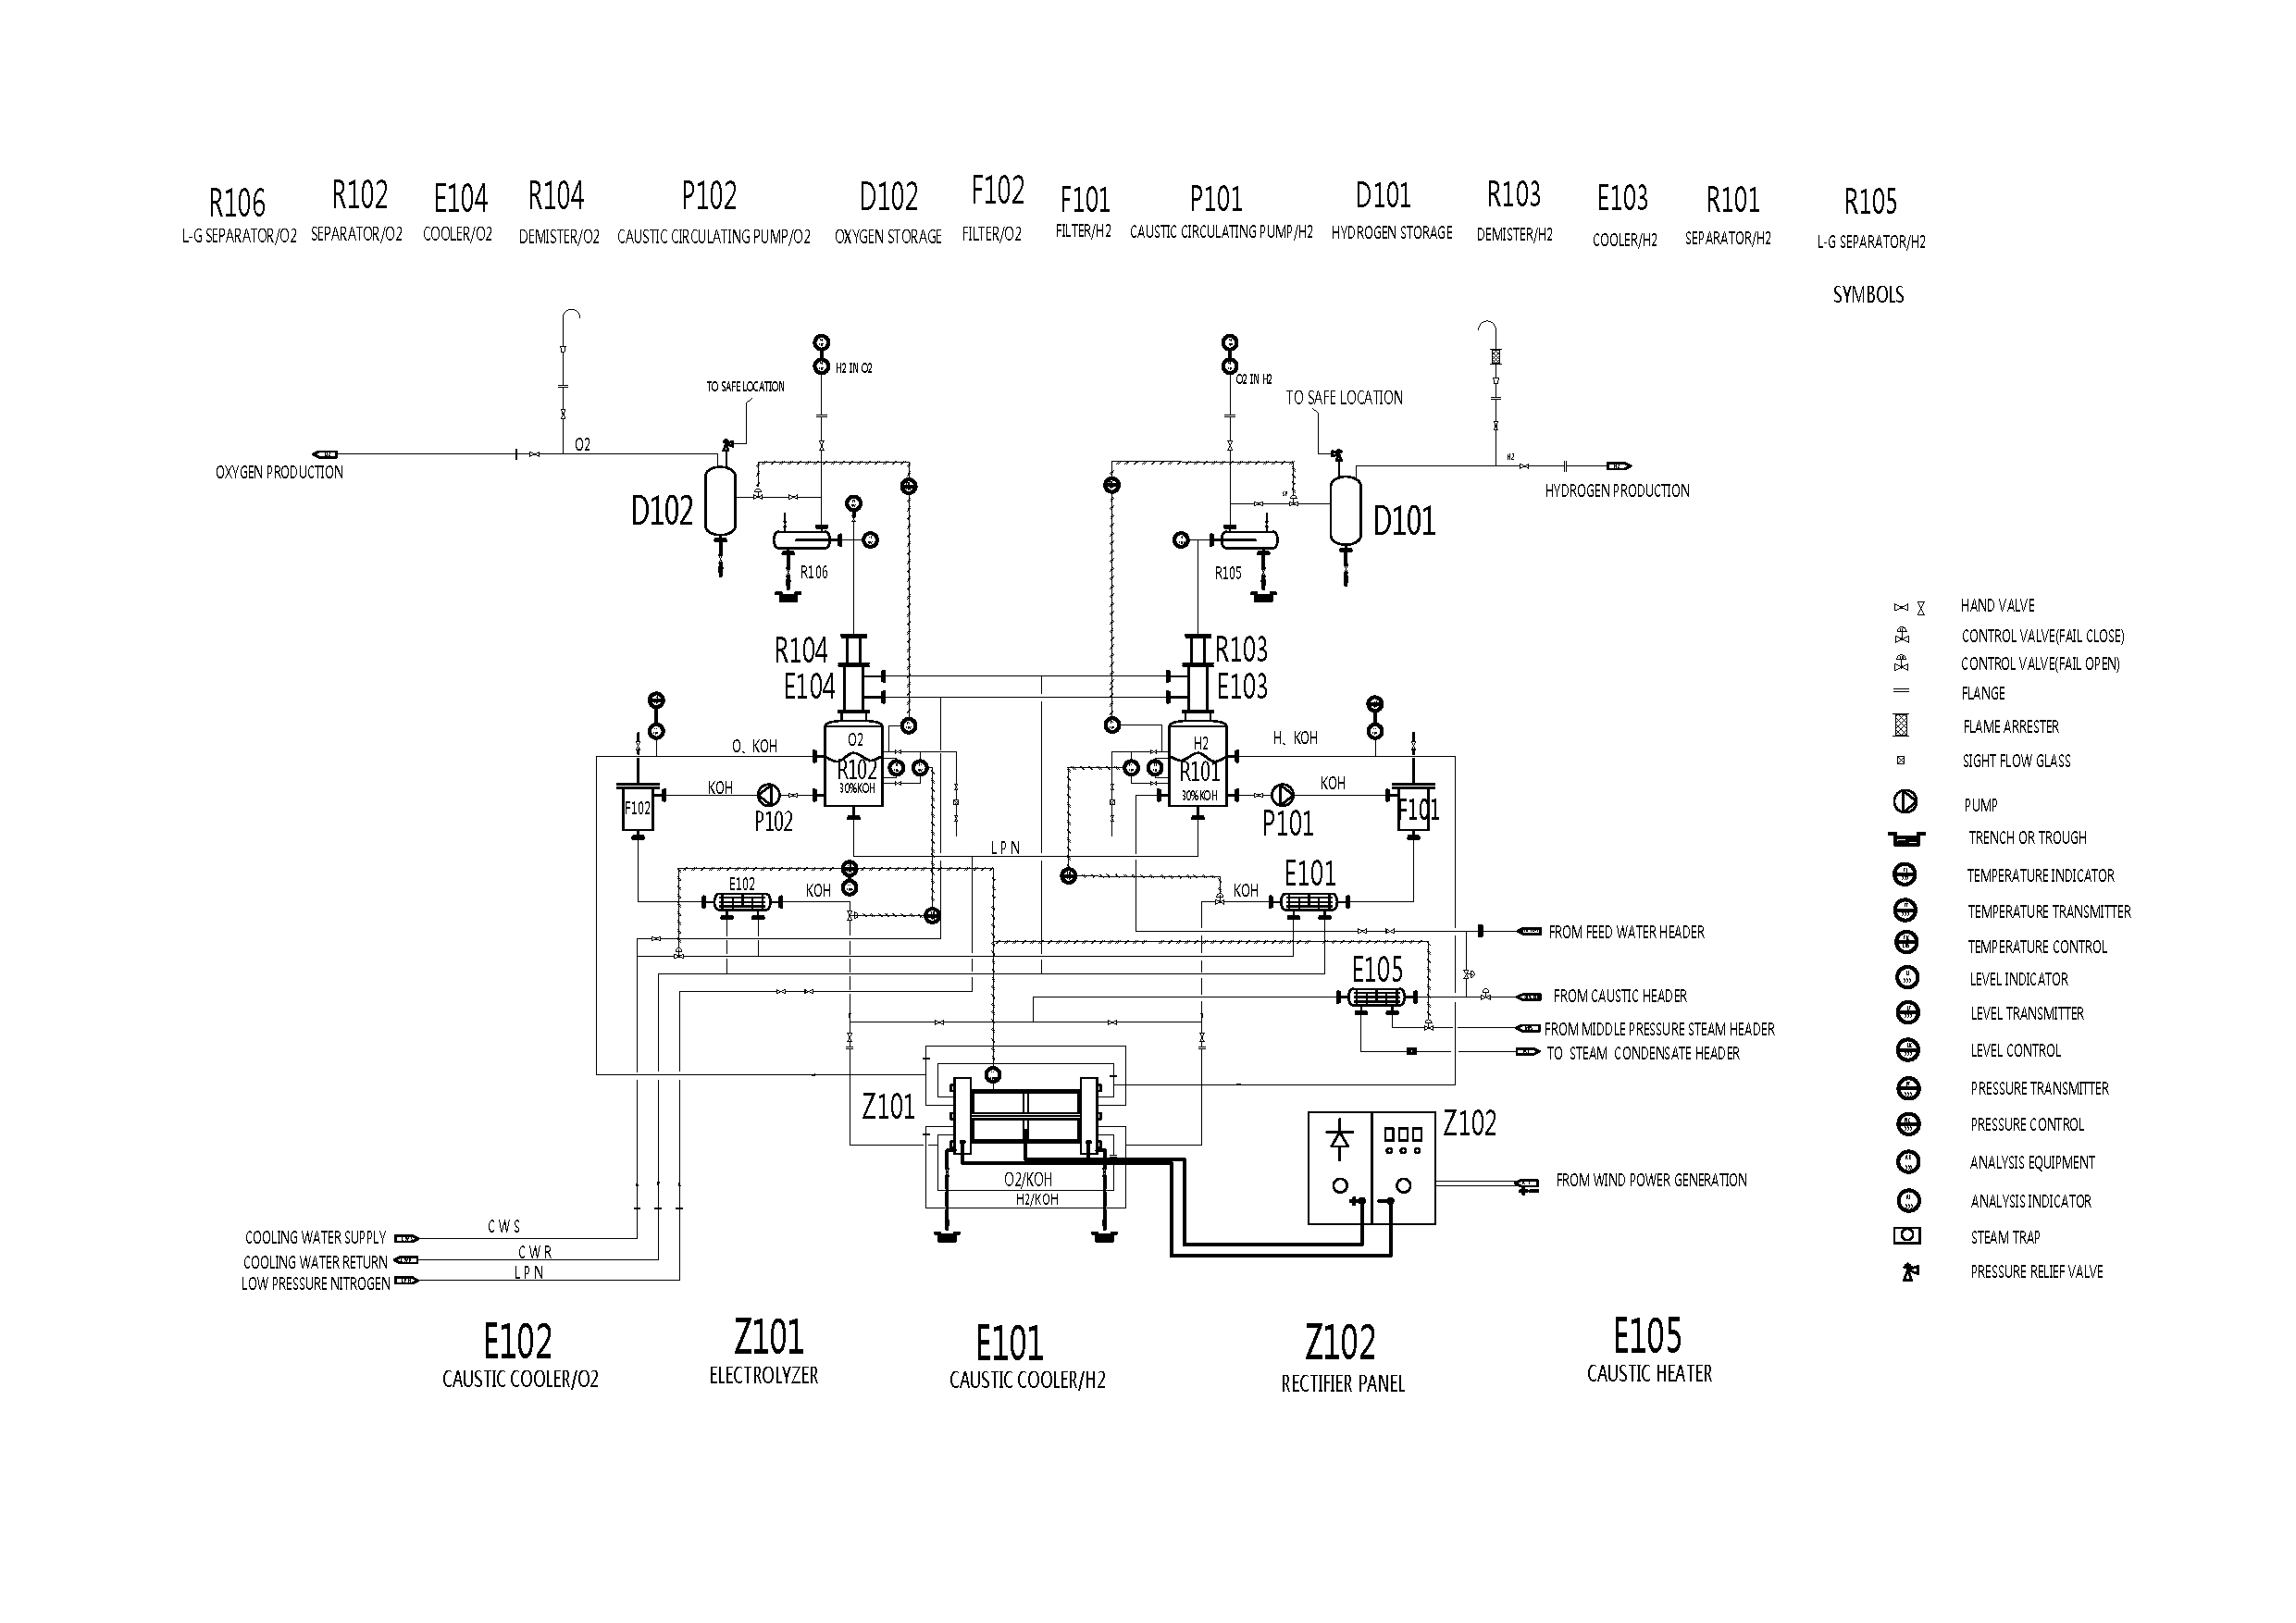
\includepdf[page=-,pagecommand={\thispagestyle{style-3yp}{cadcad.pdf}}
%\includepdf[pages=-,angle=90]{cadcad.pdf}

\subsubsection{Dynamic system response}
Because the power output from the wind farm is variable, intermittent and unpredictable, the electrolyser is required to cover a wide load range(typical load range is 100\% - 20\%). Some alkaline electrolysers can operate at a small overload, but they are not considered here because they lowers lifetime and efficiency. The lower limit is set for gas purity concerns: if the wind energy is below a minimum limit, the electrolyser can be either shut down or operate at a standby mode (energy is supplied to the stack to maintain a minimum hydrogen production rate). A complete shutdown would require a rather time-consuming start-up process while operating at the standby mode lowers efficiency, and therefore a compromise has to be made. In this model, the electrolyzers have multiple stacks that can be shut-down independently and automatically in order to reduce the minimum power input requirement and thus improve the system flexibility.  In addition, the electrolyser also needs to have a fast response in order to capture the peaks of he energy supply. Despite the dynamic nature of hydrogen production, the hydrogen consumption rate of the ammonia synthesis process is constant and therefore a hydrogen storage system is also required to store the excess energy. \cite{purity}\cite{gas} 
%?????
\subsubsection{Specification}
In industry, the typical electrical energy input efficiency is 54 kwh/$kg_{H2}$\cite{specification}. The mean hydrogen production rate is at a surplus to the hydrogen consumption rate to ensure that a constant hydrogen flow from the storage can be achieved. The water conversion rate is assumed to be 80\%. Table \ref{tab:specification} shows the flow rate and power requirement as well as the system and dynamic operation parameters. The hydrogen purity requirement is high because oxygen could adsorb on the surface of the ammonia synthesis catalyst and poison it. 
\begin{singlespace}
\begin{table}[H]
\begin{tabular}{ |c|c|c|c| } 
\hline
 \multicolumn{4}{ | c |}{Flow rates \& Power} \\
 \hline
 & $H_2$ flow rate($kmol/s$) & $H_2 O$ consumption($m^3$/h) & Power(MW) \\ 
 \hline
 Maximum & 0.71   &  65.7 &  276 \\ 
 \hline
Mean &  0.25(roughly)  & 23.6  &  99 \\ 
 \hline
 Minimum  & 0.14  &  13.1 &  55 \\
 \hline
 \multicolumn{4}{ | c |}{System \& Dynamic} \\
 \hline
 Purity & 99.5 to 99.9998 \%&  System Lifetime & 25 years\\
 \hline
Ramp-up $\%_{(full load)}$/second& 10 & Ramp-down$\%_{(full load)}$/second  &  10\\
 \hline
 Start-up time & 20min & Load range  & 20\% - 100\%\\
 \hline
\end{tabular}
\caption{System Specification} \label{tab:specification} 
\end{table}
\end{singlespace}


     
\subsection{Fundamentals} 
Electrolysis is a non-spontaneous redox reaction that is carried out in the electrolytic cell, with the electrolyser filled with electrolytes (anion and cation) to improve conductivity. When a DC current passes through the electrodes, hydrogen is produced at the cathode, and oxygen is generated at the anode, it is important to note that the metal from electrolyte should be more reactive than hydrogen, so that hydrogen is produced instead of metal. The electrolyser is divided into the anode chamber and the cathode chamber by the diaphragm, with electrodes placed in each chamber. The reaction in alkaline solution is as follows:
\begin{equation} 
Cathode \quad 2H_2 O(l) + 2e^- \rightarrow H_2(g) + 2OH^-(aq)\quad   \phi_0=-0.828V
\end{equation} 
\begin{equation} 
Anode \quad 4OH^-(aq) \rightarrow O_2(g) +2H_2O(l) +4e^- \quad \phi_0=0.401V
\end{equation} 
\begin{equation} 
The \ overall \ reaction \quad H_2O(l) \rightarrow \frac{1}{2} O(g) + H_2(g) 
\end{equation} 
The molar rate of hydrogen production for cells connected in series can be determined by considering Faraday's law, which presents as 
\begin{equation} 
\ f_{H2} = \eta_F \frac{N_{cell}I_{cell}}{zF} =\eta_F\frac{N_{cell} jA}{zF} 
\end{equation} 
where $\eta_F$ is the Faraday efficiency, F is Faraday's constant, z is the number of electrons transferred, which is 2 in this reaction. $n_c$ is the number of cells, I is total current, j is current density, and A is cell area.It is shown in the equation that the production rate is directly proportional to the current. \cite{rate} The objective is to minimise power consumption and increase efficiency, both electrochemical and thermodynamic effects should be taken into account for optimising the operation conditions.


\subsubsection{Thermodynamics} 
The electrolysis process is an endothermic reaction, the enthalpy change is expressed as
\begin{equation} 
\triangle H =\triangle G + T\triangle S = zF[T(\frac{\partial U_{rev}}{\partial T})_p - U_{rev}]
\end{equation} 
where $\triangle G $ is the Gibbs free energy change, which is the energy required to split water and is therefore the minimum electrical energy required. $T\triangle S$ represents thermal energy, $\triangle S$ is the change of the reaction entropy. $U_{rev}$ is the reversible voltage and p is the prevailing pressure (Pa). F is Faraday's constant, and z is the number of electrons transferred, which is 2 in this reaction.\cite{gibbs}  
Under standard conditions (1 atm, 25$^{\circ}$ C), $\triangle H^0 = 285.8 kJ/mol, \triangle S^0 = 163.14$. Therefore, $\triangle G^0 = 237.2 kJ/mol.$ With increasing temperature, the energy required for decomposing water is reduced. This is why high temperature electrolysis method is adopted for the electrolysis process.The minimum voltage required (the reversible voltage) can be calculated by
\begin{equation} 
U_{rev} =\frac {-\triangle G} {zF} 
\end{equation} 
The reversible cell voltage at standard condition is therefore 1.23V. In reality, the actual voltage required is usually greater than this due to irreversibility. Therefore it is also important to consider the thermoneutral voltage, which is the voltage at which the reaction is neither endothermic nor exothermic. 
\begin{equation} 
U_{tn}=\frac{-\Delta H} {zF}
\end{equation} 
At standard conditions, $U_{tn} = 1.48V.$ Between 1.23V and 1.48V, the reaction is endothermic.\cite{thermoneutral} 

\subsubsection{Reversible Voltage} 
The reversible cell voltage is the minimum potential required for water decomposition. Reversible cell voltage is a function of temperature and pressure, and can be calculated by
\begin{equation} 
E_{rev}(T,p)=E_{rev}(T) + \frac{RT} {zF}ln[\frac{p-p_w)^{1.5}p*_w} {P_w} ]
\end{equation} 
The first term represents reversible voltage at atmospheric pressure and can be shown as
\begin{equation} 
E_{rev}(T)=1.50342-9.956 \times 10^{-4}T+2.5 \times10^{-7}T^2
\end{equation} 
 The second term shows the effects of pressure due to the wet gases being in contact with the electrolyte vapour near the electrode, which is a function of electrolyte vapour pw and pure water pressure pw*. R is the universal gas constant.
 \begin{equation} 
p_w=T^{-3.498} exp(37.93-\frac{6426.32} {T} )\exp(0.016214 - 0.13802m+0.19330\sqrt{m} ) 
\end{equation} 
\begin{equation}
pw*=T^{-3.4159} \exp(37.043-\frac{6275.7} {T} ) 
\end{equation} 
where m is the molarity of the electrolyte solution, and it can be expressed as a function of temperature and  concentration by
\begin{equation} 
m(t, W_t\%) =\frac{W_t\%(183.1221-0.56845T+984.5679 \exp(W_t\%/115.96277))} {100(56.105)} 
\end{equation} 
Figure\ref{fig:Urev} shows the the effects of temperature and pressure on reversible voltage as well as the variation of pw and pw* with temperature. 

\begin{figure} [h] 
%\centering

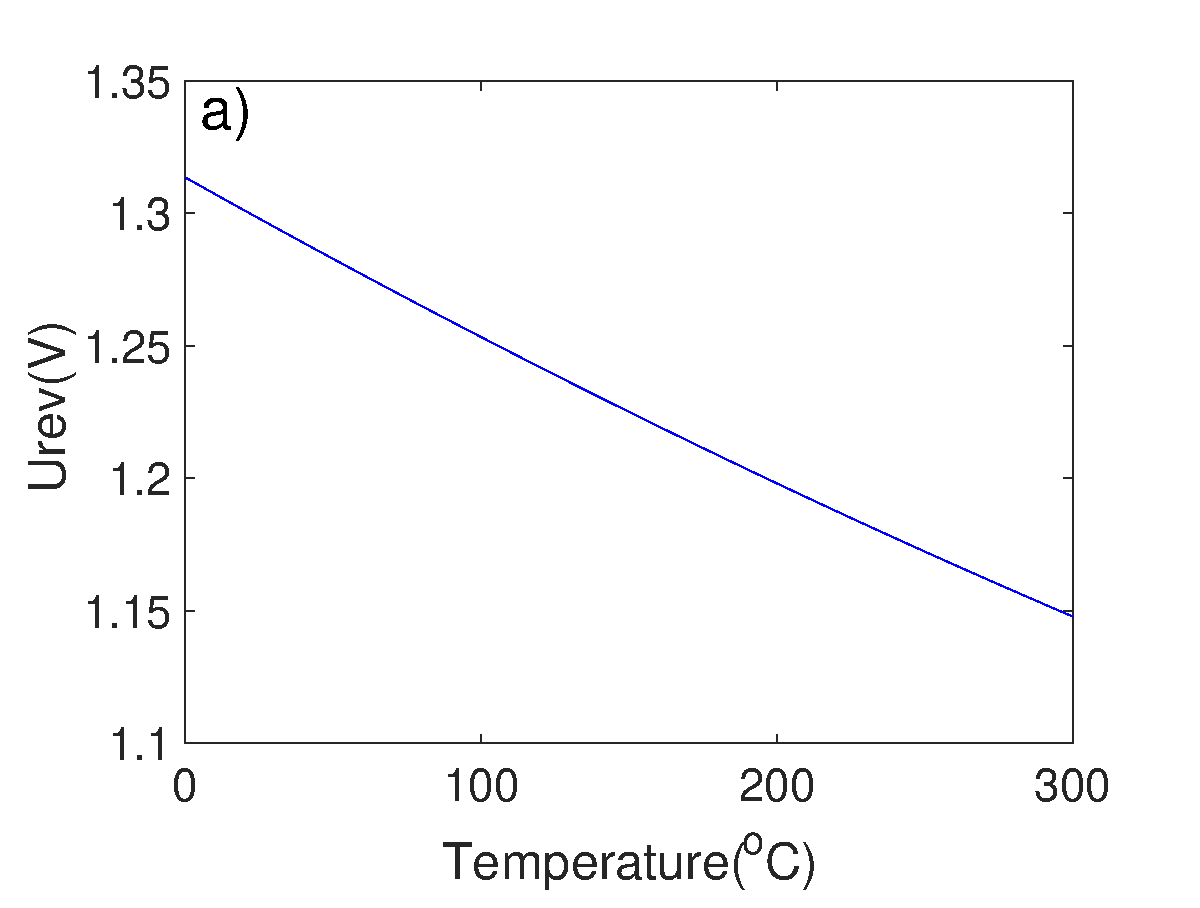
\includegraphics[width=5.5cm]{temperature.eps} 
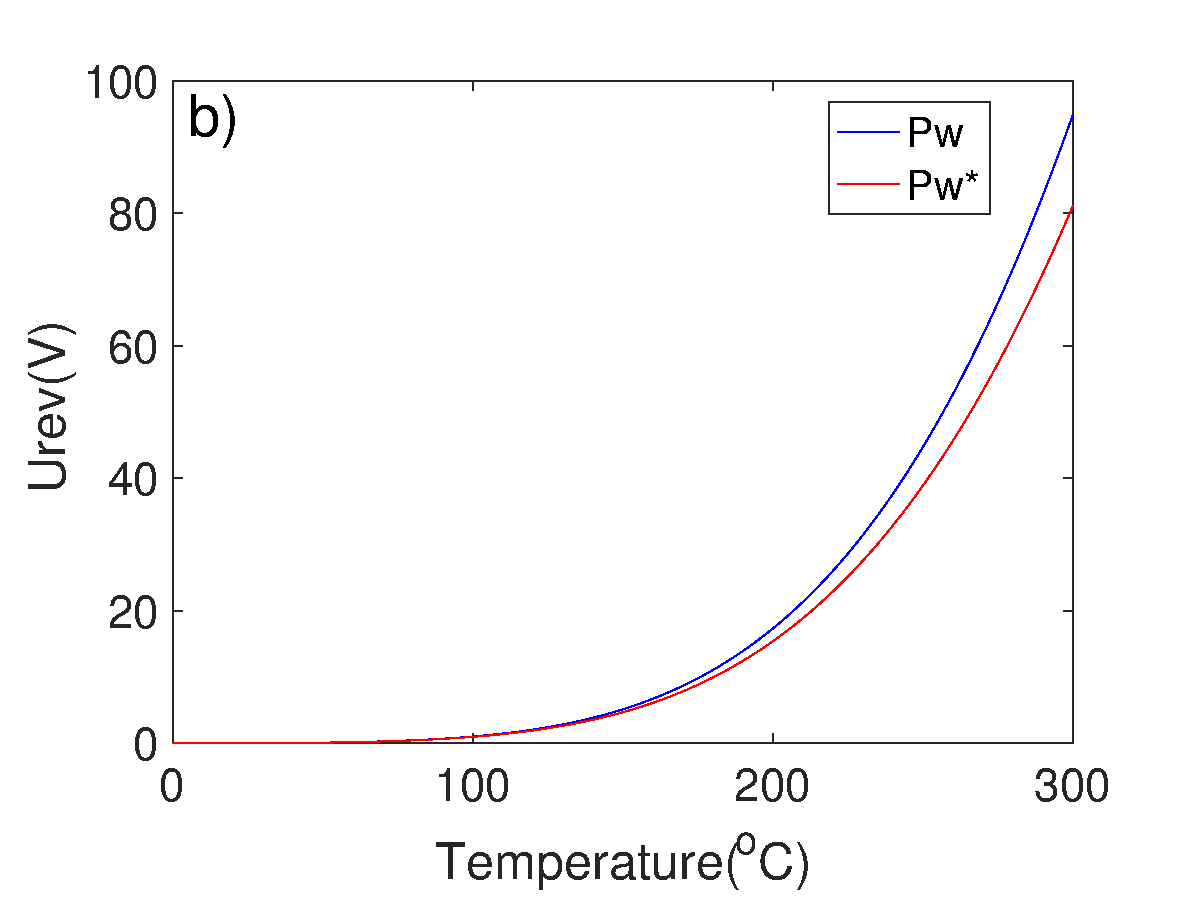
\includegraphics[width=5.5cm]{pw.eps} 
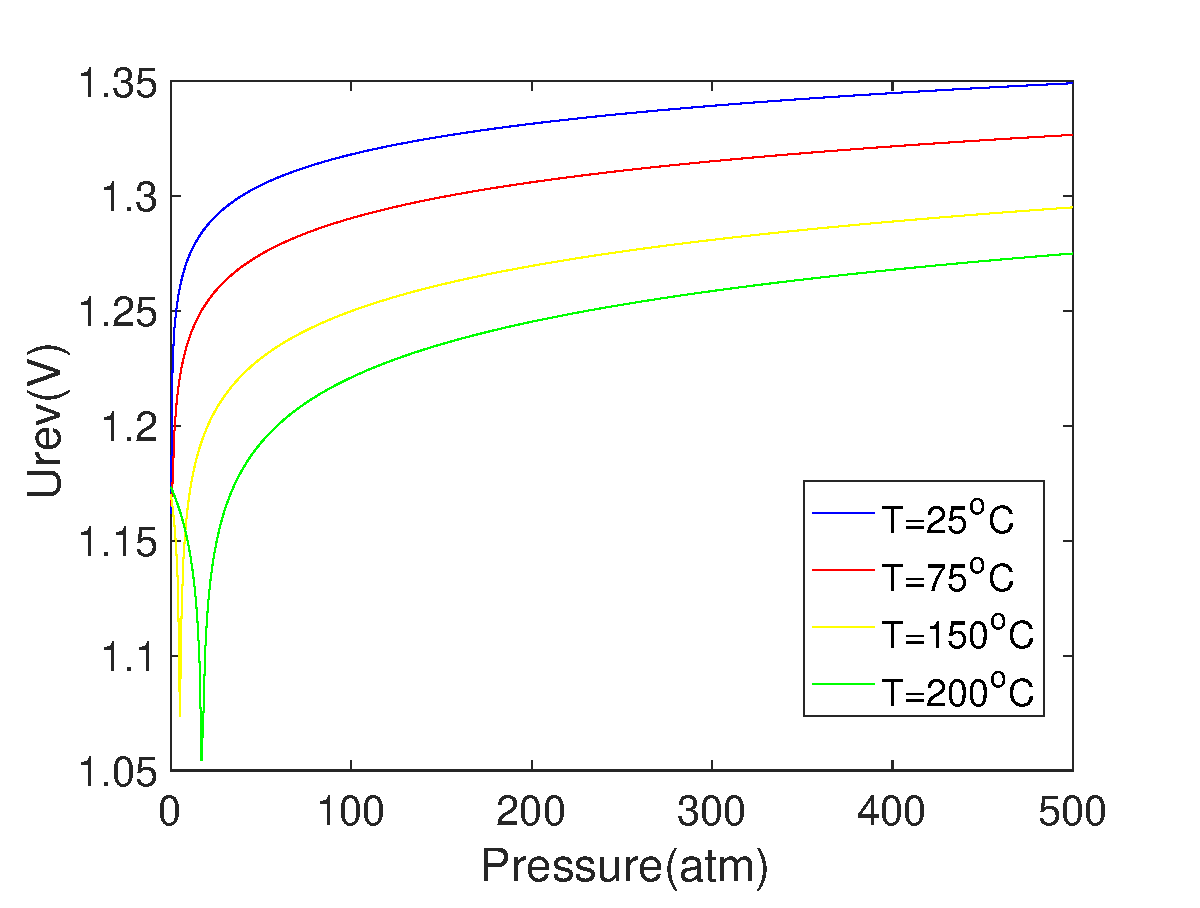
\includegraphics[width=5.6cm] {pressure.eps} 

\caption{Variation of reversible voltage with temperature(left) Pw and pw* with temperature(middle) and pressure at various temperature(right), assuming 25\% concentration} 
\label{fig:Urev}

\end{figure} 


%It can be shown from the graphs that high temperature favours the reaction, however, in the model designed, An increase in pressure also lowers the reversible voltage, although this has a much smaller effect compared with temperature. The electrolysis is carried out at elevated pressure mainly in order to increase the boiling temperature of the electrolyte and obtain pressurised hydrogen which is more energy efficient during the compression process. Real-gas behaviour also has an effect on the reversible cell voltage, however the effect is detrimental and an ideal gas behaviour can be assumed below 200 bar.\cite{reversible}
%It can be shown on Matlab that the effect of concentration changes on reversible voltage is very small. 

\subsubsection{Electrochemistry} 
The actual cell voltage would be higher than the reversible energy  as a result of irreversibility of the process. The cell voltage is the sum of reversible voltage, overpotential due to Ohmic losses, activation overpotential and concentration overpotential.
\begin{equation} 
U_{cell}=U_{rev}+U_{ohm}+U_{act}+U_{con}
\end{equation} 

%\begin{figure}[h]
%\centering
%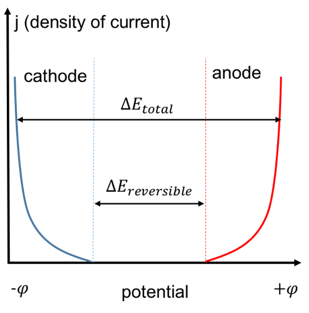
\includegraphics[width=6cm]{electrochemical.png} 
%\caption{total cell voltage and reversible cell voltage}
%\end{figure} 

\subsubsection{Ohmic Overpotential} 
Each component in the electrolytic cell can be modelled as an electrical conductor. When current passes through the conductors, there is ohmic power loss due to the resistivity of the conductors which will lead to a heating effect. Since the electrolysis reaction is endothermic, some of the heat can be utilised within the system.While most ohmic energy is lost in the electrolytic solution, the membrane, wirings, electrodes  and bubble effects also form part of the electrical resistance.The heat generated can be evaluated by  $ Q=UI=I^2 R$, where R can be computed by
 \begin{equation}
R=\frac{l} {A \kappa} 
\end{equation} 
where $ \kappa(S/m) $  is the conductivity of the solution.\newline
The total ohmic loss is the sum of all components in the electrolysis cell.
\begin{equation} 
R_{total}=R_{electric} + R_{anode}+ R_{cathode}+R_{bubble}+R_{ions} +R_{membrane} 
\end{equation} 
For the electrolytic solution, the area specific resistivity of the electrolyte can be calculated by
\begin{equation} 
r_{ions}=\frac{\delta_{el}} {\sigma_{el}(T,M) } 
\end{equation} 
where $\delta_{el}$ represents the electrolyte layer thickness and $\sigma_{el}$ represents the conductivity of the solution which varies with temperature and molarity.
The conductivity of electrolyte varies with temperature, concentration and composition. The specific conductivity of electrolyte (S/m) can be estimated by
\begin{equation} 
\sigma_{el} = (A(M) + B(M^2) + C(MT) + D(\frac{M} {T}) + E(M^3) +F(M^2T^2) )\times 100
\label{eq:sig}
\end{equation} 
where M represents the molarity in mol/L, and T is Temperature in Kelvin, and A-F are constants.\cite{conductivity}  The molarity M is related to electrolyte concentration by equation 10 stated before. 
\begin{figure}[h] 
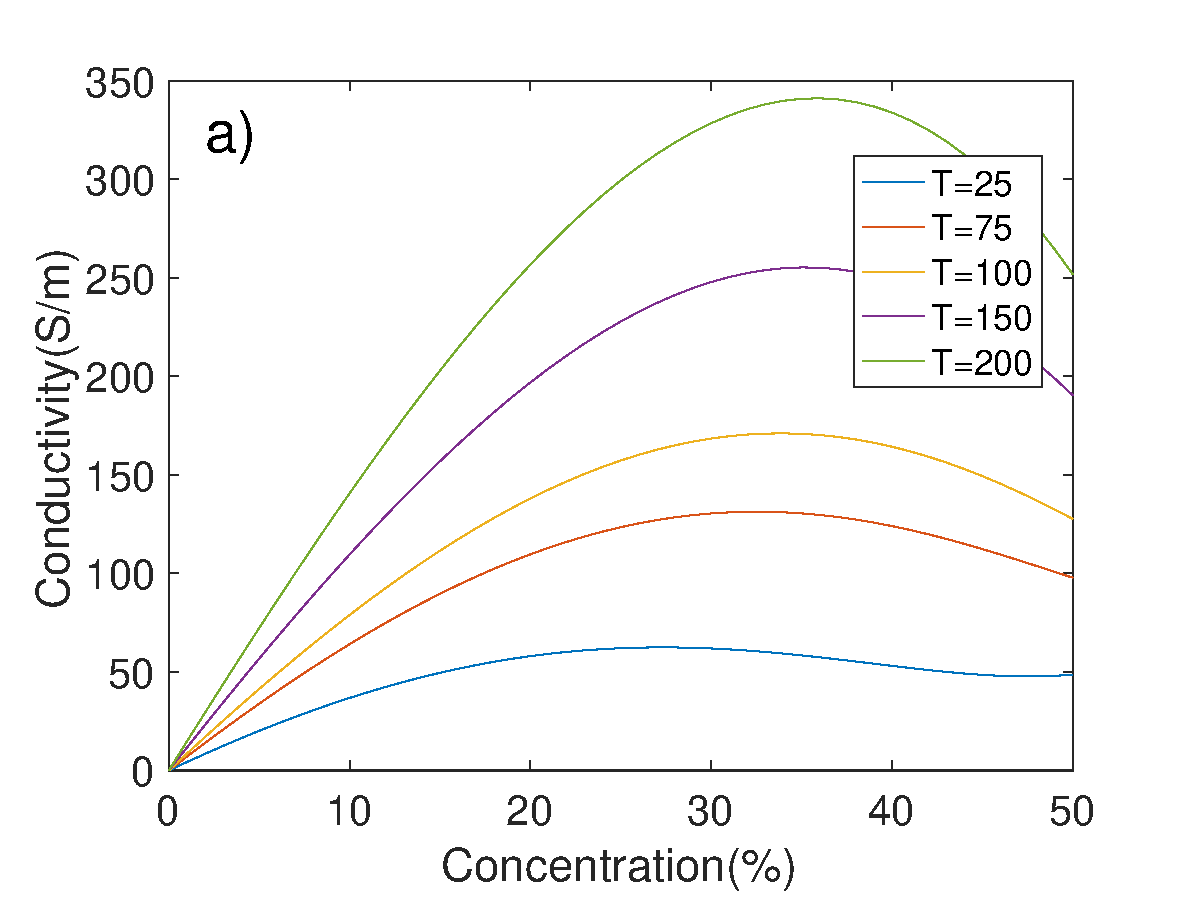
\includegraphics[width=5.5cm] {cond.eps} 
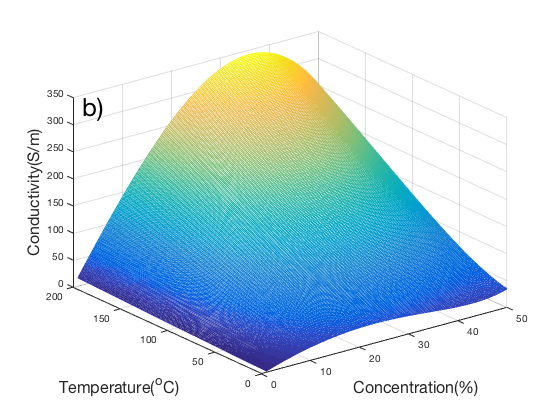
\includegraphics[width=5.5cm]{3D.eps}
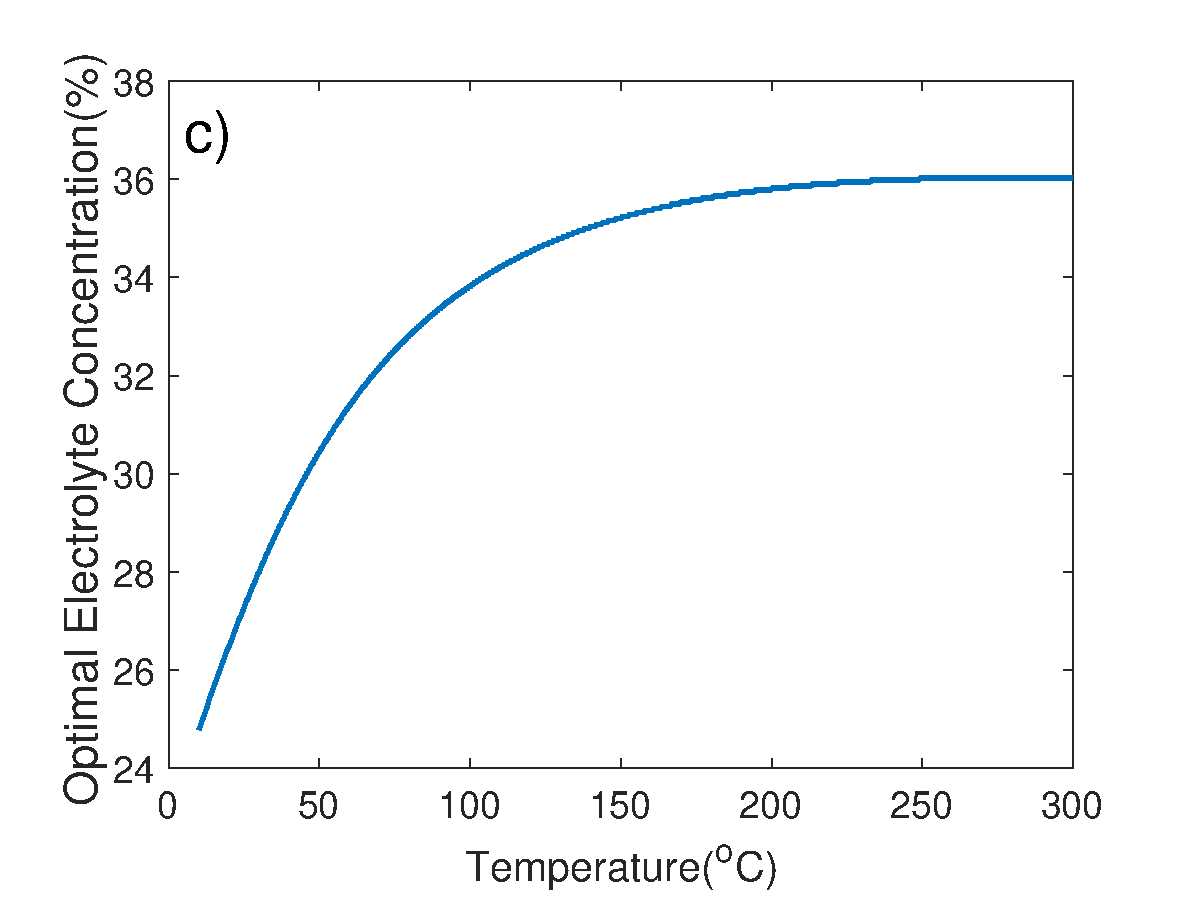
\includegraphics[width = 5.5cm]{optimum.eps}
\caption{ a)Variation of conductivity with temperature and concentration. b)3D plot. c) and the optimal concentration of electrolyte with temperature} 
\label{fig:3D}
\end{figure} 
It can be seen from Figure \ref{fig:3D} that the conductivity increases when concentration is higher, this is due to the increase in the number of unit ions per volume in the solution. However the solution does have a limit of how conductive it can reach, once that limit is achieved, the conductivity starts decreasing with increasing concentration. It can also be shown that the conductivity increases with increasing temperature, this is because an increase in temperature may also cause an increase in the number of ions in solution due to dissociation of molecules. Also noteworthy is the existence of an optimal concentration which increases with increasing temperature: at above 200 degree Celsius, the optimal concentration reaches around 36\%. In reality, however, the electrolyte concentration is usually around 25 - 30 \% because a very high concentration could lead to corrosion.
The ohmic overpotential from electrolytic solution is therefore\
\begin{equation} 
U_{ohm} = r_{ions} \times J
\end{equation} 
where J is the superficial current density. 


%The conductivity is further decreased due to bubbles effects, The conductivity can be calculated using Bruggeman correction
%\begin{equation} 
%\sigma_B= \sigma_0(1-\alpha_{total} )^{1.5} 
%\end{equation} 
%where $\sigma_0$ is the conductivity with no bubbles and $\alpha_{total} $is the total void fraction.
 %overpotential is a specific form of concentration overpotential and is due to the evolution of gas at either the anode or cathode. This reduces the effective area for current and increases the local current density. The bubbles located on or very near to the elecuode surface contribute significant electrolyte conductivity loss because their population is very crowded at the gas evolving surface.

 %Which depends upon several factors including the rate of gas evolution at the electrode  $\frac{\dot{V_G}}{A}$ ,  the average residence time of bubbles at the electrode surface $t_r$, and the average bubble volume at departure from the electrode surface $V_r$.
%\begin{equation} 
%\Theta = \frac{\pi} {2} \frac{\dot{V_G}} {A} \frac{t_r}{V_r}{R_r} ^2
%\end{equation} 
%where $R_r$ is the bubble radius at detachment
%\begin{figure}[h] 
%\centering
%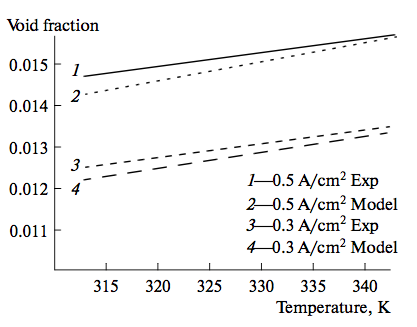
\includegraphics[width=10cm] {void} 
%\caption{Comparisons between experimental and modeling results } 
%\end{figure} 

%The electrode can be considered as a resistor in parallel with a capacitor, The space between the electrodes should be reduced to reduce the ohmic loss and to make the current density higher. For instant, the distance between electrodes is a typical example of less than 1 millimeter, known as a zero gap configuration method. Some manufactures commercial electrodes and membranes as the only components to make batteries, so that the real zero gap is achieved. \cite{zerogap}

%\begin{figure}[h] 
%\centering
%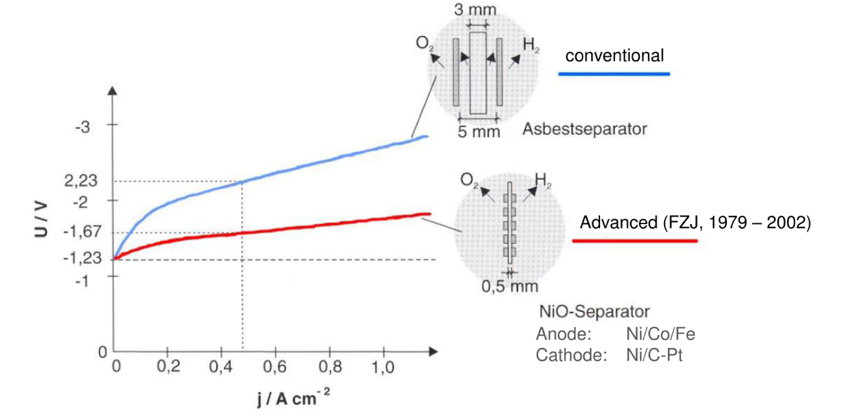
\includegraphics[width=10cm] {zerogapgap.png} 
%\caption{UI curve for different electrode distance \cite{zerogap} }
%\end{figure} 

\subsubsection{Resistance of the Membrane}
The authors in  gave an empirical fitting of the resistance of the 0.5mm Zirfon based membrane and the temperature,
\begin{equation}
R_{mem} = \frac{0.06+80e^{T/50}}{10000S_m}
\end{equation}
Where Sm is the membrane surface in $cm^2$.

\subsubsection{Activation Overpotential}
In reality, the efficiency of alkaline electrolysis is further reduced by electrode kinetics, making the actual electrode potential higher than the reversible potential. The difference is called the activation overpotential. This represents the kinetic barriers that need to be overcome for the gas evolution reactions at each electrode. Various experiments have shown that the overpotential for oxygen evolution reaction (OER) is much higher than for that the hydrogen evolution reaction (HER), and it depends heavily on the catalytic properties of electrode materials. \cite{activation} There are many other factors that influence the overpotential, including temperature, current density, concentration and impurity of the solution.
The corresponding current density can be calculated using the Butler-Volmer equation. \cite{activation1}
\begin{equation} 
J = J_0 [e(^{\frac{\alpha_a}{RT}zFU_{act,a}}) - e(^{\frac{\alpha_c}{RT}zFU_{act,c}})],
\end{equation}
where J is the current density, $J_0$ is the exchange current density, which represents current at equilibrium, the oxidation and reduction reaction rates are opposite and equal, resulting in zero net current, and  $\alpha_{a/c}$ is the charge transfer coefficients. The charge transfer coefficients are related by temperature by
\begin{equation} 
\alpha_a = 0.0675 + 0.00095T, \alpha_c = 0.1175+0.00095T
\end{equation} 
For large overpotential, this can be approximated by the Tafel equation\cite{activation2} 
\begin{equation} 
U_{act,a/c} = 2.3026 \frac{RT}{zF\alpha_{a/c}} log(\frac{J}{J_0}).
\end{equation}
The exchange currents density is found experimentally, which can be significantly different depending on the electrode composition and temperature. It has been determined by Wendt and Pizak that for steel blasted nickel electrodes at $90^oC$, the exchange current density at anode and cathode are $7.9 \times10^{-3}Am^{-2}$ and $7.1Am^{-2}$ respectively. \cite{activation3} The activation overpotential can be decreased by using catalysts, and this will be discussed later in the report. The activation overpotential at cathode and anode and the effects of temperature are shown in Figure \ref{fig:activation} . It can be shown that the activation overpotential increases with temperature, but this effect is quite small.
\begin{figure}[h] 
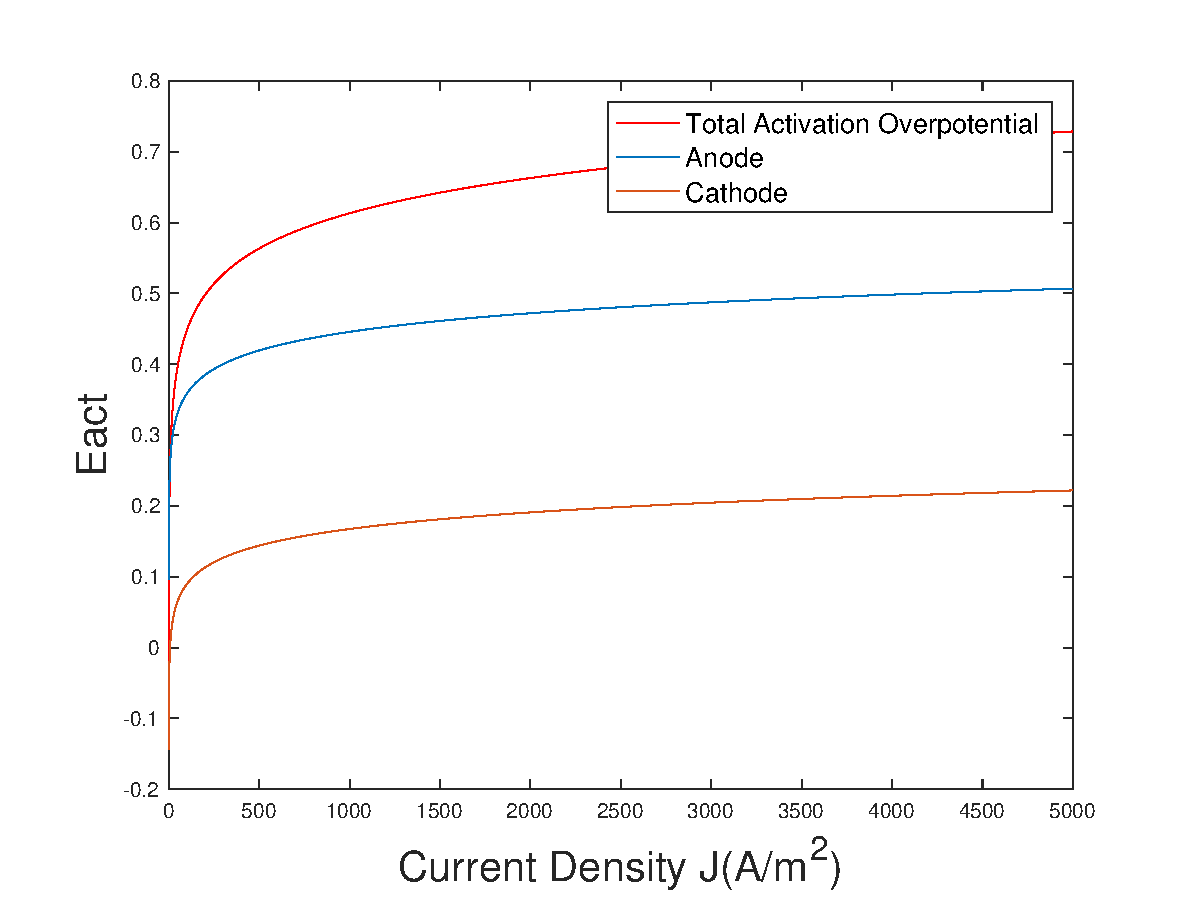
\includegraphics[width=8cm] {Activation.eps} 
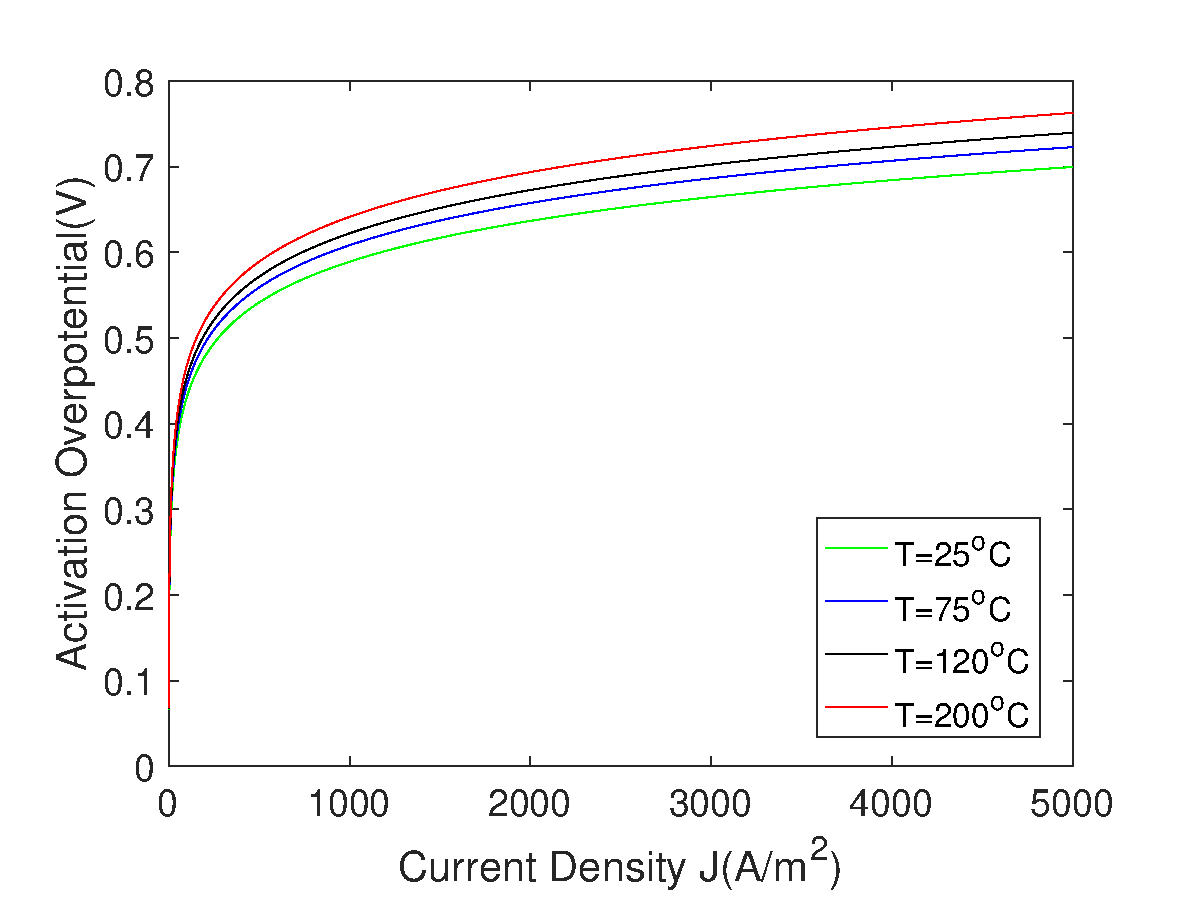
\includegraphics[width=8cm]{ActivationT.eps}
\caption{Activation Overpotential at cathode and anode(left),effects of temperature(right)} 
\label{fig:activation}
\end{figure} 

\subsubsection{Bubble Effects}
When hydrogen and oxygen are produced at the electrodes, the bubbles will partially adhere to the electrodes, making a fraction of the surface electrochemically inactive so that current is applied to a smaller area. The effective surface area of the electrodes is
\begin{equation} 
S_{eff} = S(1-\theta)
\end{equation}
As a result, the actual current density is greater than the superficial one, their relationship is,
\begin{equation} 
Ja = \frac{J}{S_{eff}} = \frac{J}{1-\theta}
\end{equation} 
where Ja is the actual current density, J is the superficial current density, and $\theta$ is the bubble coverage ratio on electrode surface, with values between 0 and 1. An empirical equation has been developed from experimental data that relates bubble coverage and superficial current density \cite{bubble2} 
\begin{equation}
\theta = 0.023(\frac{J}{Am^{-2}})^{0.3}
\end{equation} 
Apart from current density, the bubble coverage also depends upon several other factors including the rate of gas evolution at the electrode surface, and the average residence time of bubbles at the electrode surface , and the average bubble volume at departure from the electrode surface.\cite{bubble2} The total activation potential combined with bubble effects can be calculated by\cite{activation4} 
\begin{equation} 
U_{act-\theta} = 2.3026\frac{RT}{zF\alpha_{a/c}}{log(\frac{J}{J_0}}) - 2.3026log(1-\theta) 
\end{equation} 
where the second term on the RHS represents the bubble effects. Another important effect of bubble formation is  the reduction of electrolyte conductivity, which will increase the ohmic resistance of the electrolyte. The effective conductivity  can be calculated using the Bruggman equation\cite{void} 
\begin{equation}
\sigma_B = \sigma_0(1- \alpha_{total})^{1.5}
\end{equation}
where $\alpha_{totoal}$ is the void fraction, which is the fraction of volume occupied by the gas. $\sigma_0$ is the conductivity without any bubbles and $\alpha_{total}$ is the total void fraction. Unlike many other models  that were developed from assuming equal-sized spheres, the Bruggman model was derived assuming many different bubble sizes.  As can be seen from figure 7(c), the conductivity reduces rapidly with increasing void fraction. Take temperature $= 120^oC$ for example, a void fraction of 0.37 halves the conductivity. %The voltage loss as a result of conductivity reduction can be calculated by\cite{void2}
%\begin{equation}
%V_{ohm} = \frac{\delta_{el} J_{av}}{\sigma_B}
%\end{equation}
%where $J_{av}$ is the average current density, and $\delta_{el}$ is the electrolyte layer thickness.
The void fraction is related by bubble coverage by\cite{activation2}
\begin{equation}
\alpha_{total} = \frac{2}{3}\theta
\end{equation}

\begin{figure}[h] 
\centering
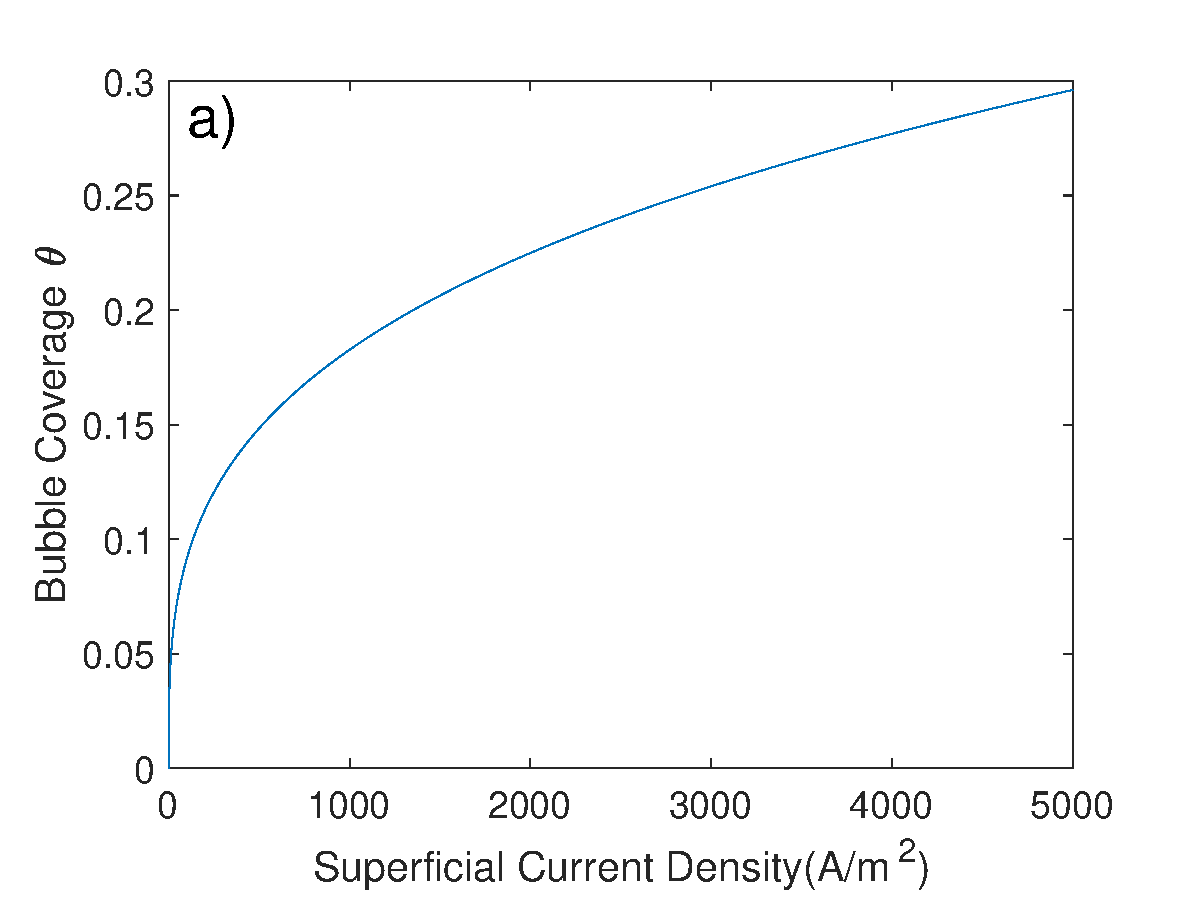
\includegraphics[width=7cm]{coverage.eps}
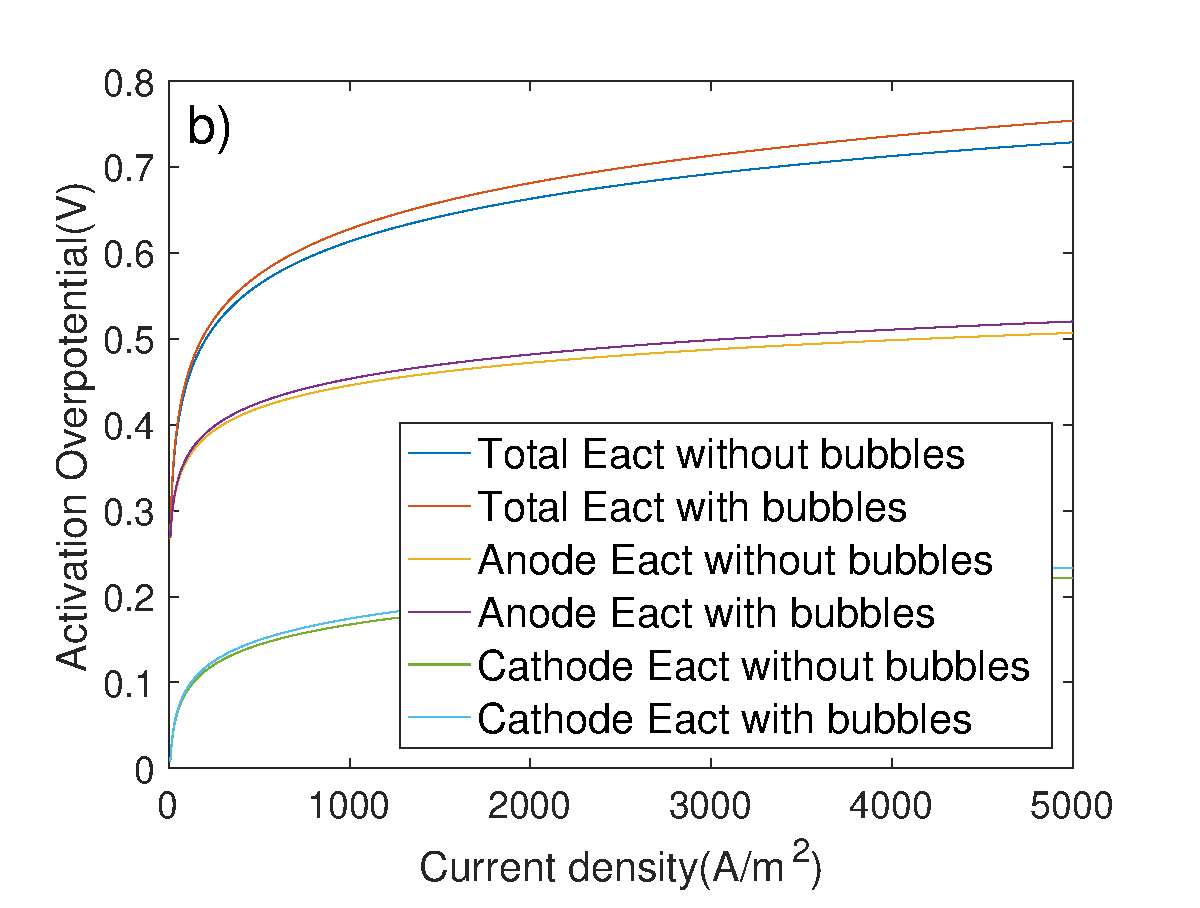
\includegraphics[width=7cm] {actbubble.eps} 
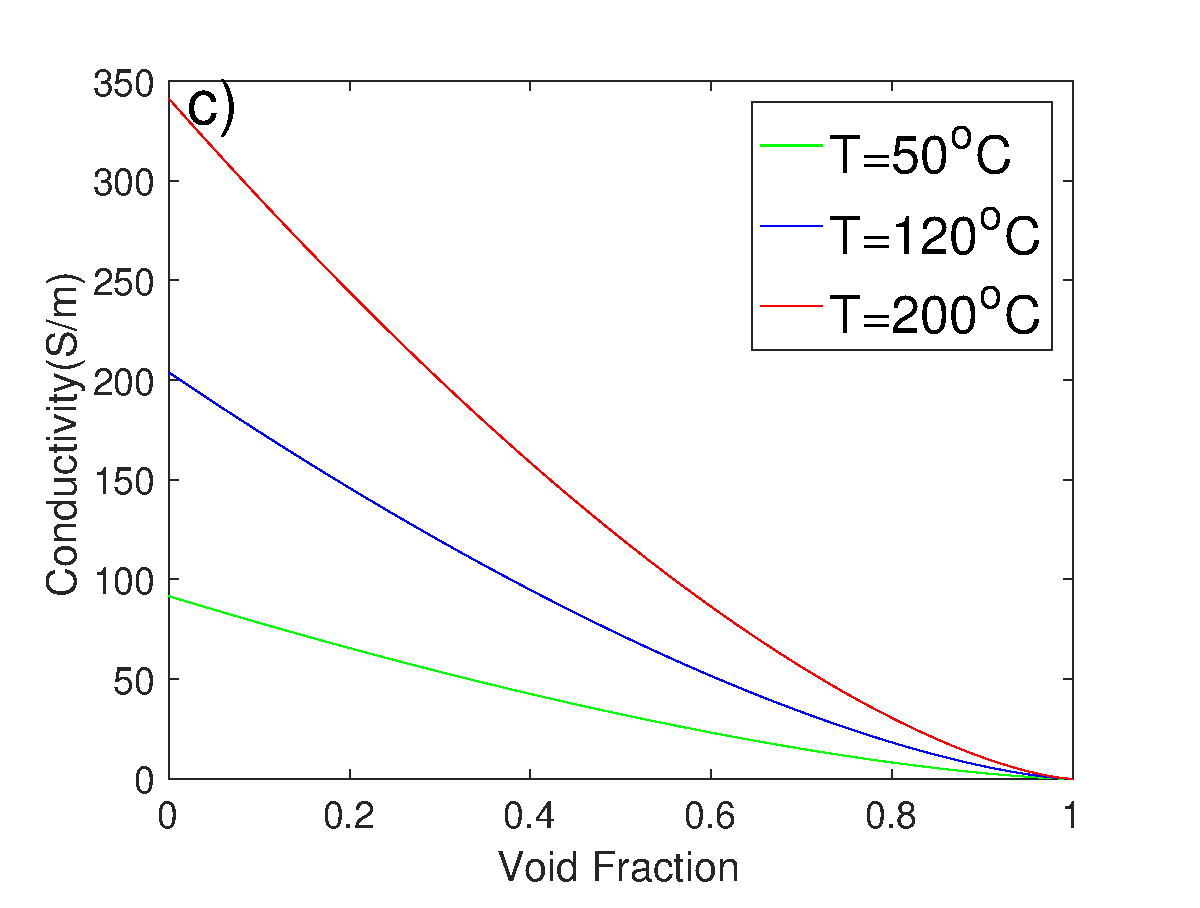
\includegraphics[width=7cm]{void2.eps}
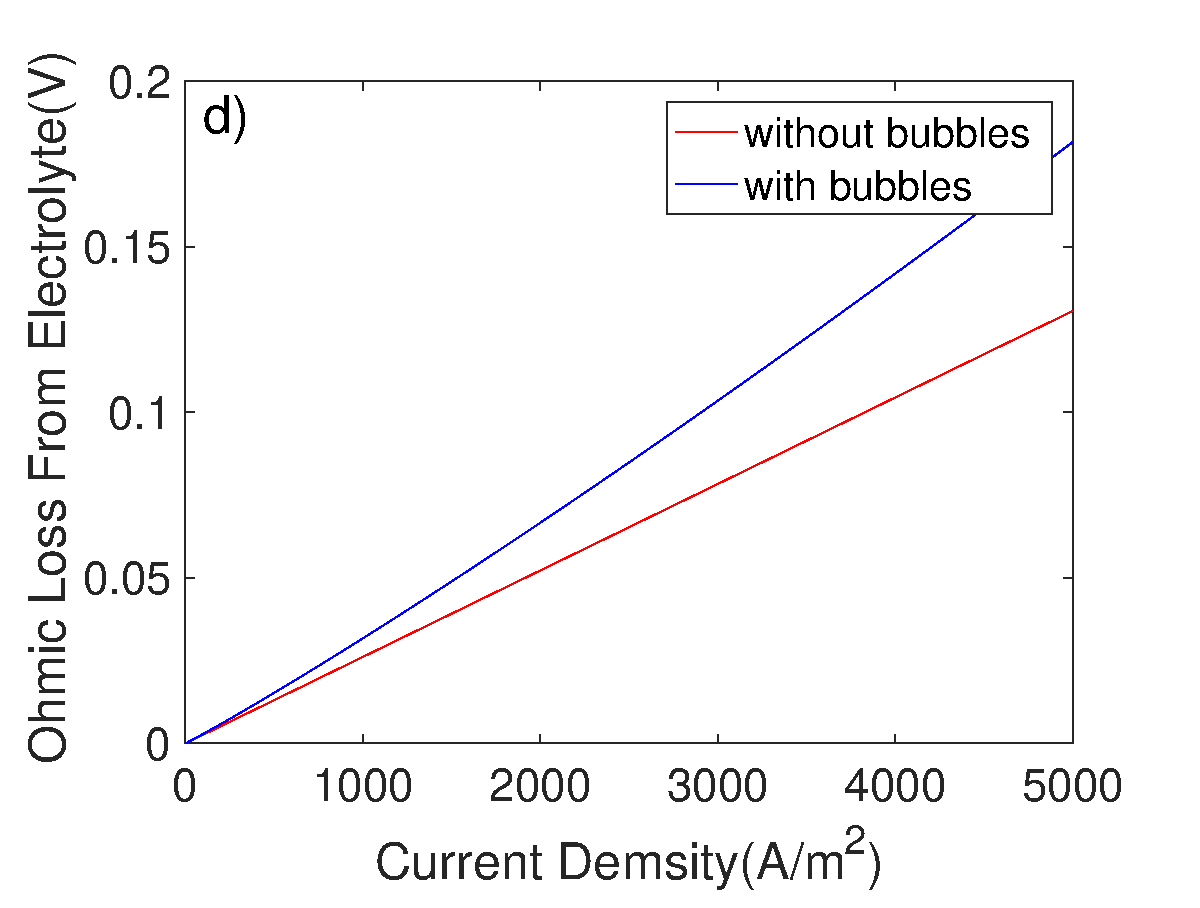
\includegraphics[width=7cm]{bubble3.eps}
\caption{a)Bubble coverage against current density. b) Activation Overpotential taking into account the bubble effects at electrodes against current density. c)Conductivity against void fraction d) Ohmic voltage loss from electrolyte with and without bubbles} 
\end{figure} 



\subsubsection{Overall Cell Voltage and Optimum Operating Conditions}
The polarisation curve of the alkaline electrolysis cell is plotted in figure 8 a), it is observable that the total cell voltage increases with higher current density. This is largely due to the increased contribution from ohmic losses,especially from bubble formation, whereas the curve for activation polarisation actually becomes flatter at higher current density. This means that a lower current density will lower the energy consumption and thus increase the system efficiency. However, the hydrogen production rate, which increases with higher current density,  is also an important factor to consider along with the system efficiency.  Electrolyser degradation and safety issues also influence the choice of current density. The rate of electrolyser degradation increases rapidly with higher current density and this will thus increase the investment cost. The large amount of heat produced as a result of higher current density, if poorly managed, can be dangerous. In addition, gas crossover is more significant at low current density, and this is because although the amount of gases crossing over the membrane remains the same, there are smaller amounts of gases produced to dilute the effects. The result is a highly flammable mixture once it reaches a certain limit. In industry, a compromise has to be made. The current density is usually kept between 1000 - 3000$A/m^2$. \cite{currentdensity}\cite{currentdensity2}

\begin{figure}[h]
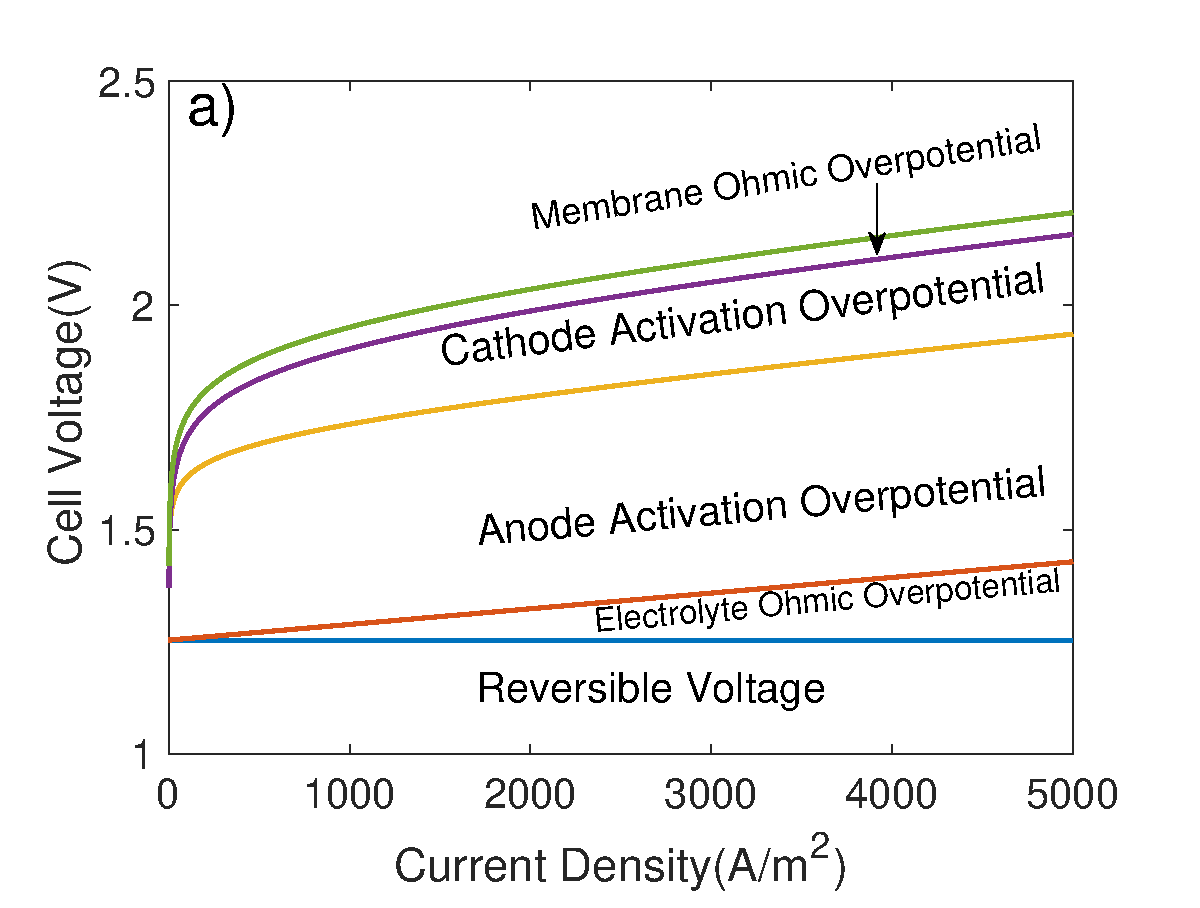
\includegraphics[width=5.5cm]{total.eps}
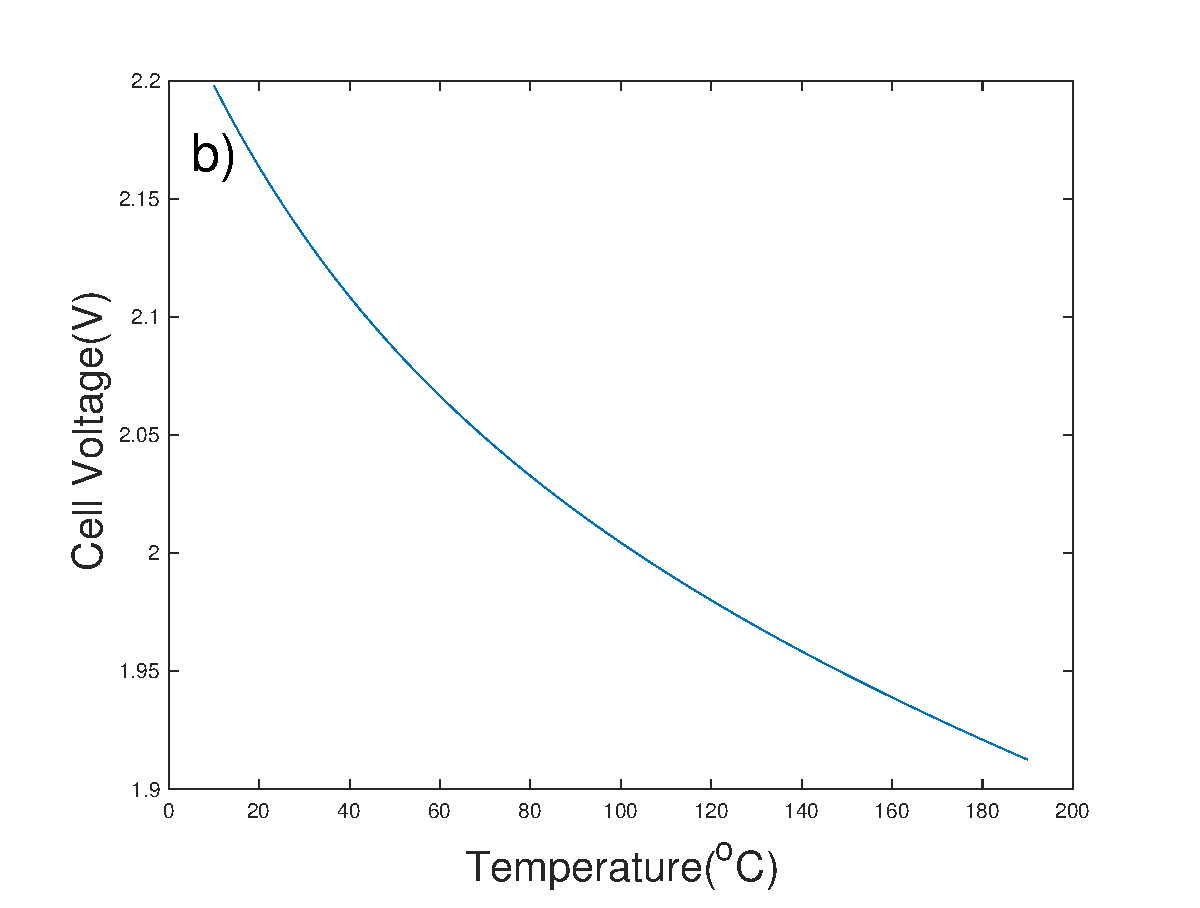
\includegraphics[width=5.5cm]{cellT.eps}
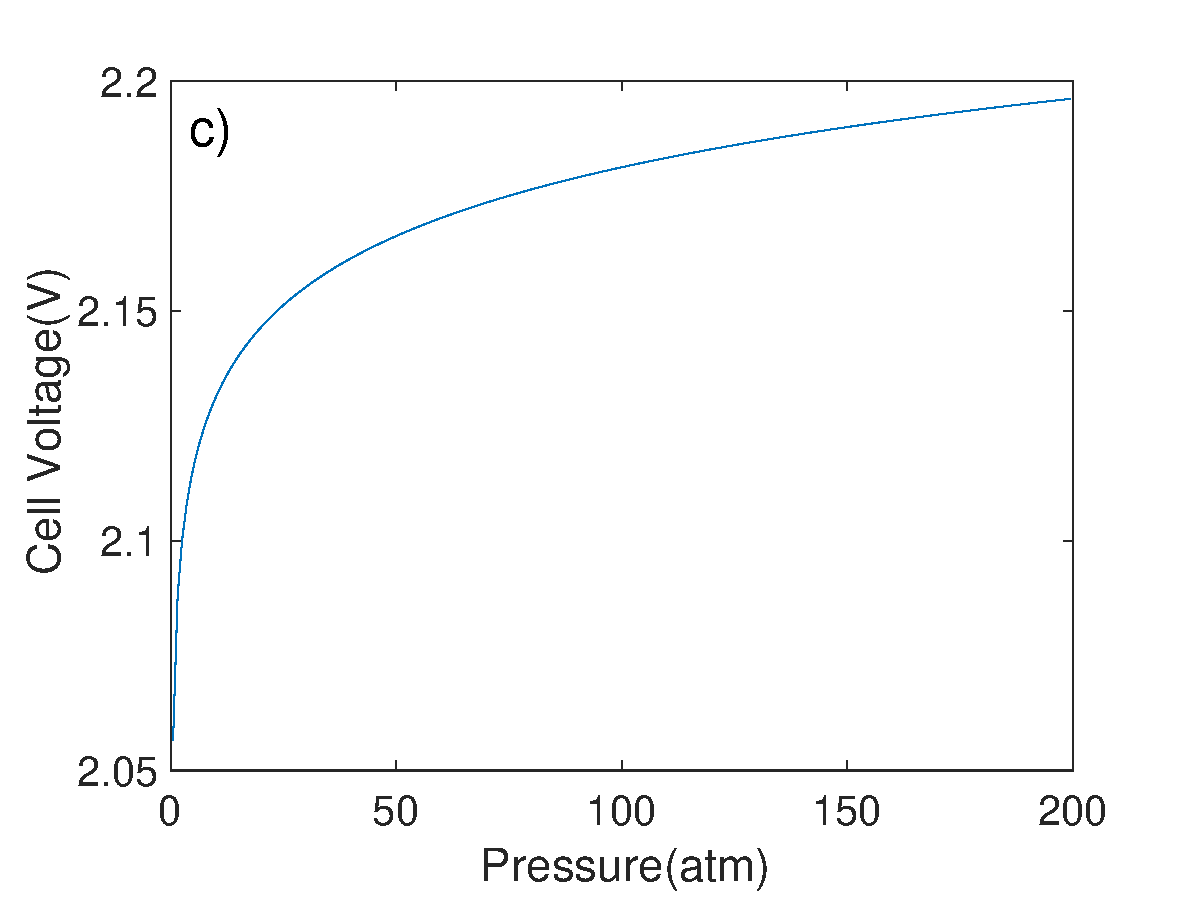
\includegraphics[width=5.5cm]{cellP.eps}
\caption{a)Total cell voltage showing cumulative effects of reversible voltage, activation and ohmic overpotential. b)Total cell voltage against temperature. c)Total cell voltage against pressure}
\label{fig:}
\end{figure}
Raising the operating temperature is one of the most effective ways to improve efficiency. As can be seen in Figure 8 b), increasing the operating temperature reduces the cell voltage, as a result of decreased reversible voltage, higher ionic conductivity, and lower activation overpotential due to enhanced electrode surface kinetics. However, a high temperature means that more energy is needed to cool down the system after the separator, and high temperature can also lead to high corrosion risk which will require more expensive materials. Also, the water loss from evaporation also increases with higher temperature. Conventional electrolysis system is operated around 80 - 90$^oC$, just below the boiling point of water. There are two major ways to further elevate the operating temperature, the first way is to use a pressurised system which will increase the boiling point of electrolyte, and in industry this is usually kept at 120-150$^oC$. The second way is to carry out steam electrolysis which can increase the temperature even further to a level of above 500$^oC^.$ However this method has not become commercialized in industry due to its high economic cost.\cite{temp} \cite{reversible} \\
Pressure is another very important parameter, increasing operating pressure has several positive effects apart from allowing for higher operating temperature.  A high pressure would reduce the size of bubbles, and gases increase in solubility with increased pressure. This will reduce the ohmic loss from bubble formation. Obtaining pressurised hydrogen is also more energy efficient during the compression process. Also, higher operating pressure makes the process of hydrogen drying easier. However, at high pressure, there is more gas crossover due to diffusion since the partial pressure of both gases have increased. A high pressure also slightly increases the operating cell voltage. \cite{pressure} In industry, 
hydrogen production at a pressure of up to 30 bar is  commercial available, and this can be achieved by using a feed-water pump.\cite{pressure2} 


\subsubsection{Electrolyser Efficiency }  
Efficiency is one of the key design objectives for the electrolysis system. There are three main efficiencies to consider depending on how the system is assessment. The voltage efficiency is the proportion of effective voltage for water decomposition to the overall cell voltage
\begin{equation}
\eta_{voltaic} = \frac{E_{anode} - E_{cath} }{U_c}
\end{equation}
A more commonly used expression is the Faradic efficiency, which relates the reversible voltage to the overall cell voltage, it also represents the percentage of the actual to theoretical hydrogen production. Its value is usually lower than 1 which means that there exist the consumption of energy that does not contribute to the hydrogen production due to the parasitic currents in the system. The maximum value of the Faraday efficiency is usually above 0.95.
\begin{equation}
\eta_{Fradic} = \frac{\Delta G}{zFU_c} = \frac{U{rev}}{U_c} 
\end{equation}
The thermal efficiency takes into account the thermal energy and can be calculated by
\begin{equation}
\eta_{Thermal} = \frac{\Delta H_{t,p}}{zFU_c} = \frac{U_{th}}{U_c} 
\end{equation} 
where $\Delta H_{t,p}$ is the enthalpy change of water decomposition. The thermal efficiency is 100\% if the cell voltage is equal to the thermoneutral voltage. When cell voltage is higher than $U_{th}$, the efficiency is lower than 100\%, and the process is exothermic. A thermal efficiency of over 100\%, which is when the cell voltage is below the thermoneutral voltage,  is theoretically achievable in high temperature steam electrolysis but is generally unpractical for alkaline electrolysis system. Under standard conditions, $U_{rev} = 1.23V$ and $U_{th} = 1.48V$. The relationship between $U_{rev}$ and $U_{th}$ against current density is plotted in figure.
\begin{figure}[H]
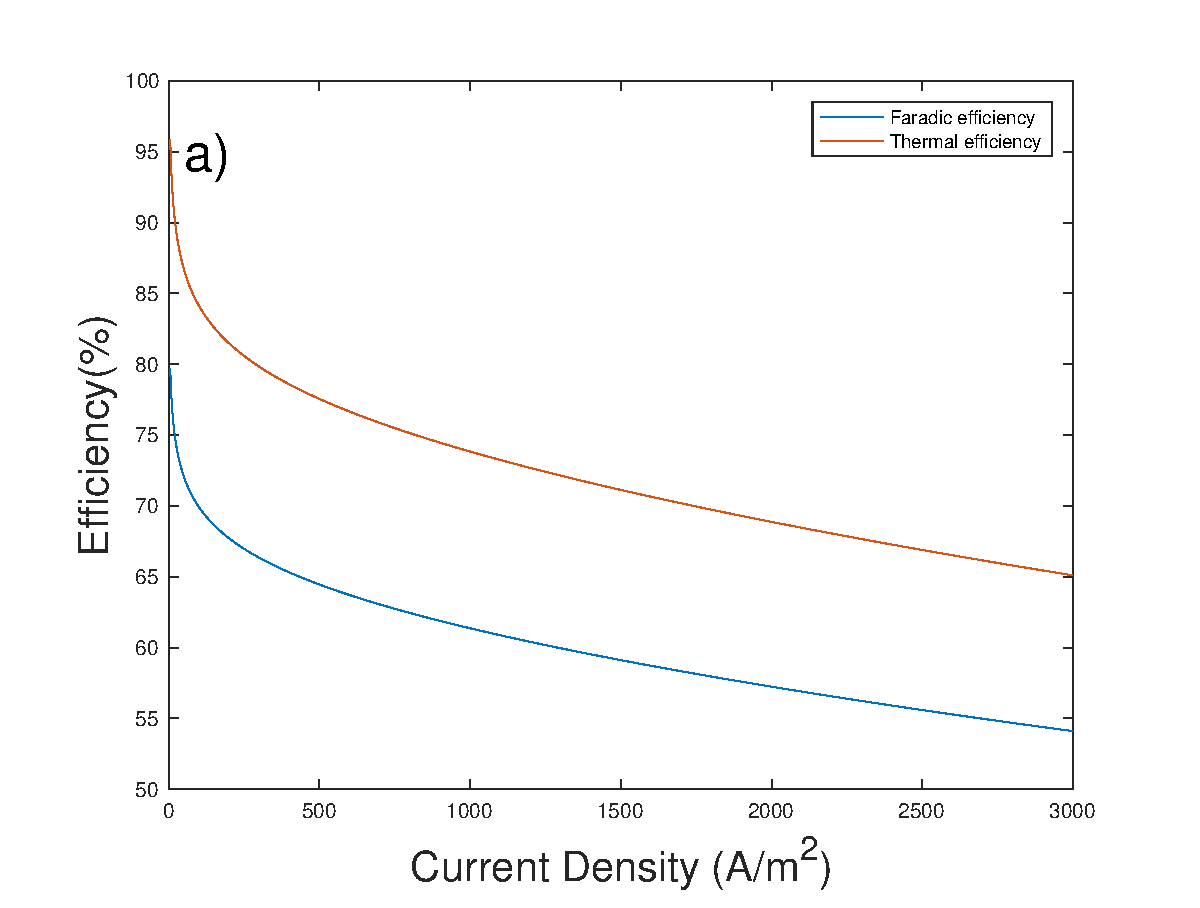
\includegraphics[width=8cm]{efficiency.eps} 
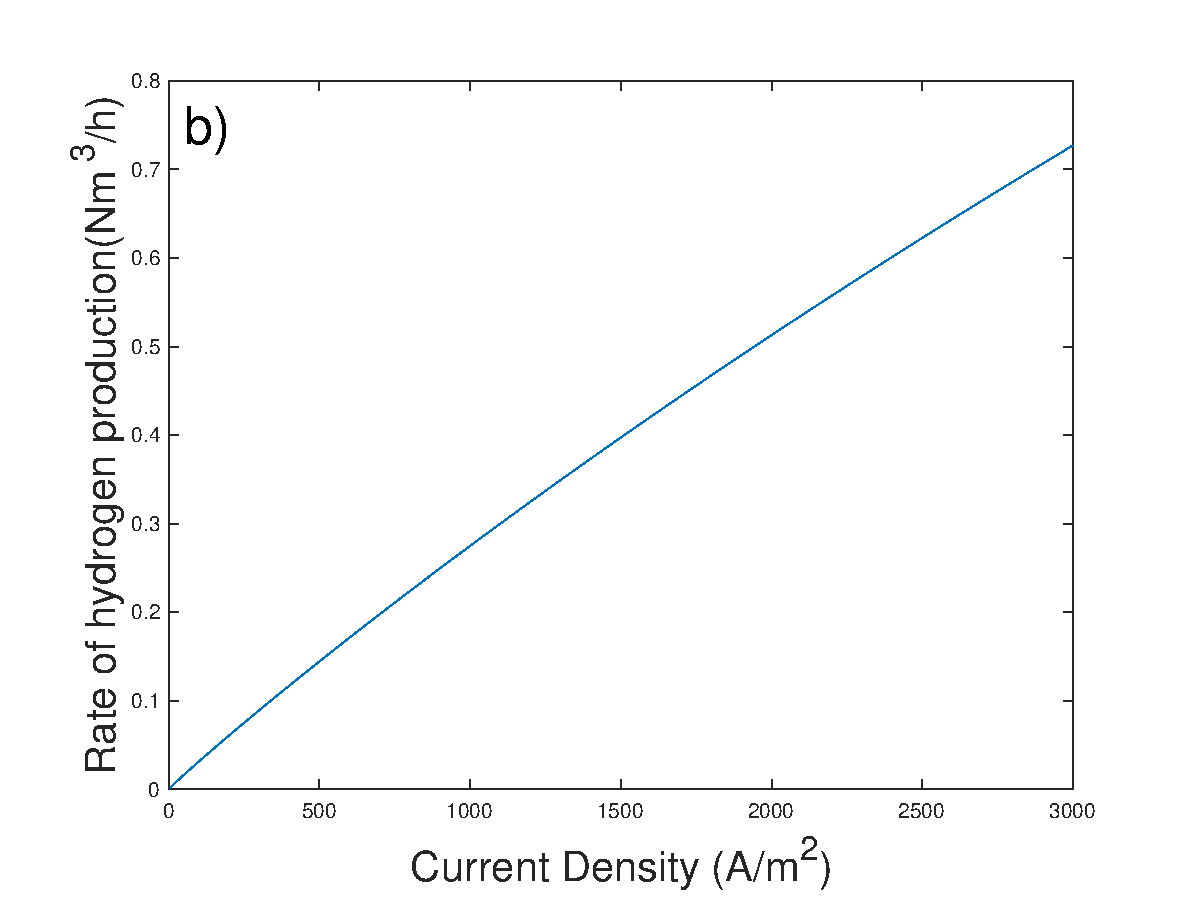
\includegraphics[width=8cm]{rate.eps}
\caption{a)Comparison of Faradic and Thermal efficiency. b)Hydrogen production rate for a single cell}
\end{figure} 

As discussed before, a high efficiency is not the only objective for this system, and a compromise has to be made between efficiency and hydrogen production rate. The rate of hydrogen production is shown in equation 4, and it can also be expressed in $Nm^3/h$ as
\begin{equation} 
 f_{H2} = \eta_F \frac{N_{cell}I_{cell}}{zF}\frac{22.41}{1000}3600
\end{equation} 
Another important parameter for the electrolysis process is the specific energy consumption,which can be calculated for a given time interval t as
\begin{equation}
C_E = \frac{\int_{0}^{t} N_{cell}  {I_{cell}}  V_{cell} dt}{\int_{0}^{t} f_{H2}dt}
\end{equation}

Finally, the electrolyser efficiency or the HHV efficiency can be calculated using the specific energy consumption by
\begin{equation}
\eta_E = \frac{HHV of Hydrogen}{C_E} 
\end{equation}
where HHV is the higher-heating-value of hydrogen.It assumes that the energy absorbed by water can be released and reused in the system by converting water back to its initial standard conditions. However, recovering the full higher-heating value is not practical in reality.
The electrical-energy efficiency can be calculated using the higher-heating voltage.\cite{efficiency} \cite{efficiency2} 
\begin{equation}
\eta_E=\frac{V_{HHV}}{V_{cell}}
\end{equation}

\begin{figure}[H]
\centering
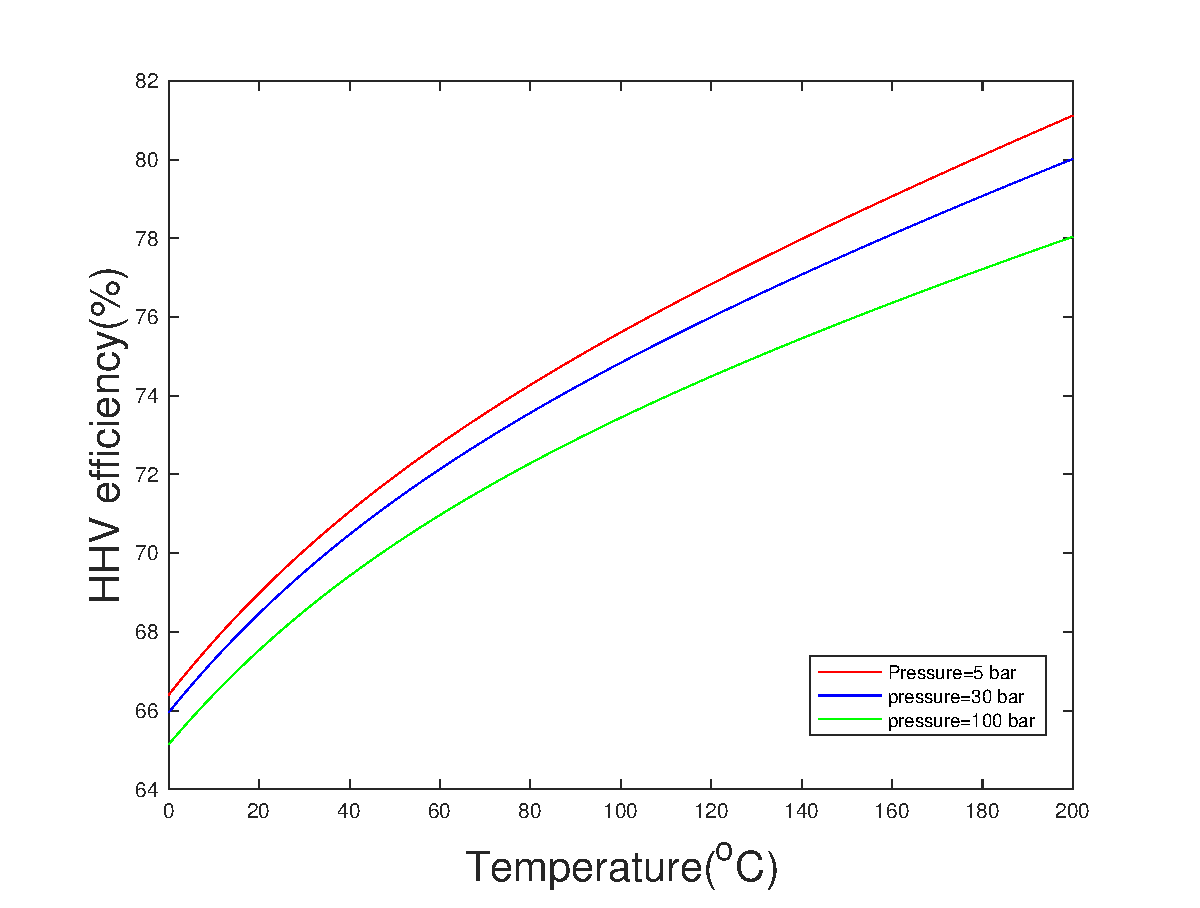
\includegraphics[width=8cm]{HHV.eps}
\caption{Variation of HHV efficiency against temperature at different pressure}
\end{figure} 
The electrolyser efficiency at different temperature and pressure with fixed current density is shown in figure, It can be seen that the electrolyser efficiency increases with increasing temperature and decreases with pressure.

\begin{table}
\centering
\begin{tabular}{ |c|c| } 
 \hline
 Temperature & $120 - 150 ^oC$  \\ 
 \hline
 Cell area & $1m^2$\\
 \hline
 Pressure & 30 bar \\
 \hline
 Number of cells per stack & 245\\ 
 \hline
 Minimum/Maximum current density & 1500/5000 $A/m^2$\\ 
 \hline
 Membrane thickness & 0.5mm\\ 
 \hline
 Minimum/Maximum Cell voltage & 1.98/2.25V \\ 
 \hline
 Electrode thickness & 2cm\\
 \hline
 $\eta_F$ at Minimum/Maximum load & 62\%/ 56\% \\ 
 \hline
 Electrode height & 45cm\\
 \hline
 $\eta_{Thermal}$at Minimum/Maximum load & 75\%/67\% \\ 
 \hline
 Electrolyte and Concentration & KOH $30\%$\\
 \hline
 HHV efficiency at Minimum/Maximum load &  76\%/68\% \\ 
 \hline
 Minimum/Maximum Flow rate(per cell) & 0.0048$mols^{-1}$/0.0145$mols^{-1}$\\
 \hline
\end{tabular}
\caption{\label{tab:table-name}Operating conditions and key parameters.}
\end{table}




%From Faraday?s law, the hydrogen production rate is proportional to the current I which represents the charge transfer in an electrolysis cell, Assuming that the same current flows through every electrolyzer cell, the hydrogen production rate in Nm3/h can be expressed as
%\begin{equation} 
%f = \eta_F \frac {NI} {zF} 
%\end{equation} 
%Where N the number of cells, I the current of cell, $\eta_F$ is the Faraday efficiency which represents the percentage of the actual production to theoretical production, its value is usually lower than 1 which means there exists the consumption of the energy that does not contribute to the hydrogen production.The maximum value of the Faraday efficiency is usually above 0.95A. Also, the electrolyser efficiency $\eta_E$ should be taken into account. It can be calculated as the ratio betwwen HHV of hydrogen and energy consumption.


\subsection{Electrolyser Design} 
%\subsubsection{Wind Power Generation System} 
 %The configuration of the wind power generation sys-tem considered in this study is shown  below:
%In order to get the Maximum Power, the system will use wind turbine's Maximum Power Point Tracking method. MPPT is a fully electronic system that varies the electrical operating point of the modules so that the modules are able to deliver maximum available power. Power captured from wind can be calculated using
%\begin{equation} 
%P=\frac{1}{2} \pi \rho C_p(\lambda , \beta)R^2v^3
%\end{equation} 
%where $\rho$ is the density of air, $\ C_p $  is power coefficient, R is blade radius, $\lambda$ is tip-speed ratio, $\beta$ is pitch angle, and v is the speed of wind.
%The wind power E, produced by rotor rotating, is 
%\begin{equation} 
%E= \frac{1} {2} m V^2-\frac{1}{2} m{V_2}^2 = \frac{1}{2}\rho AV_1(V^2-{V_2}^2) 
%\end{equation} 
%where V is the wind speed before the wind turbine, V1 is the actual speed through the wind turbine, V2 is the speed after the wind turbine. A is the Rotor section.
%In order to get the Maximum Power, the system will use wind turbine's Maximum Power Point Tracking method. MPPT is a fully electronic system that varies the electrical operating point of the modules so that the modules are able to deliver maximum available power.  So the output power of wind turbine power system is shown below

%\begin{figure}[h] 
%\centering
%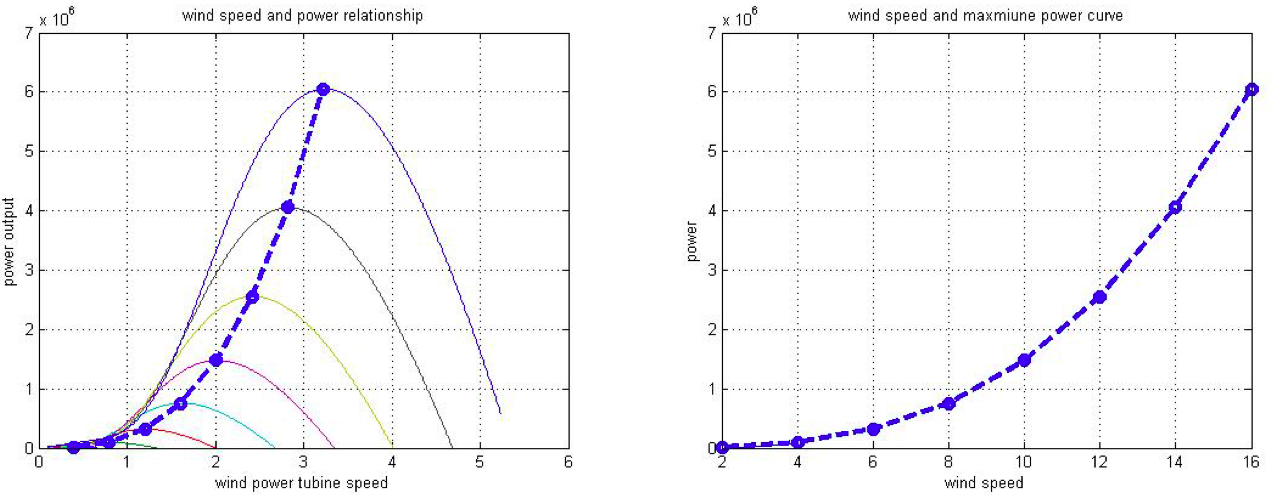
\includegraphics[width=12cm] {wind.png} 
%\caption{Wind speed and Maximum Power} 
%\end{figure} 

\subsubsection{Configuration} 
Currently there are two kinds of electrolyser configuration: unipolar and bipolar. In a unipolar configuration(or tank-type), the electrodes with the same polarity are connected in parallel, therefore the total cell voltage is the same as the voltages of individual cells, and the total current is the sum of currents in each cell. A bipolar electrolyser usually has a larger number of cells with the electrodes connected in series, and the electrodes each has both the positive and negative polarities. So current is the same in each cell and at the terminals. Unipolar electrolysers operate at a low voltage level of 1.9 - 2.5 V, but they require a high level of current. On the other hand, bipolar configuration requires a low current but a voltage of $V_{cell} \times (n-1)$, which is about 35-600V. $V_{cell}$ is the voltage for each cell and n is the number of electrodes. The industrial electrolysers are mostly bipolar electrolysers.
The pros and cons of each type of configuration are shown in table 2.

%The compact structure of the bipolar electrolyzer reduces the loss caused by the resistance of the electrolyte, thus improving the efficiency of the electrolyzer. But on the other hand, the bipolar electrolyzer has increased the complexity of design because of its compact structure, resulting in the manufacturing cost higher than that of the monopole electrolyzer. In view of the current emphasis on conversion efficiency, the industrial electrolyzer is mostly bipolar electrolyzer.

\begin{figure}[H] 
\centering
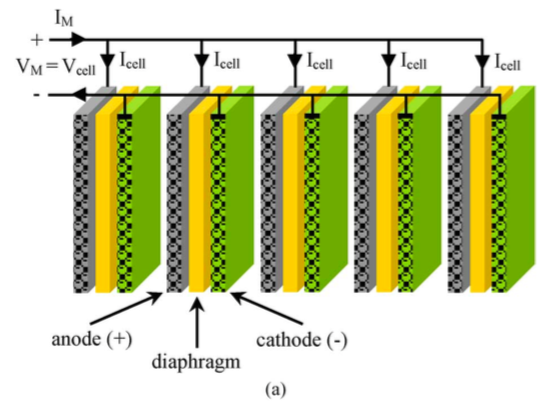
\includegraphics[width=7cm] {monopolar.png} 
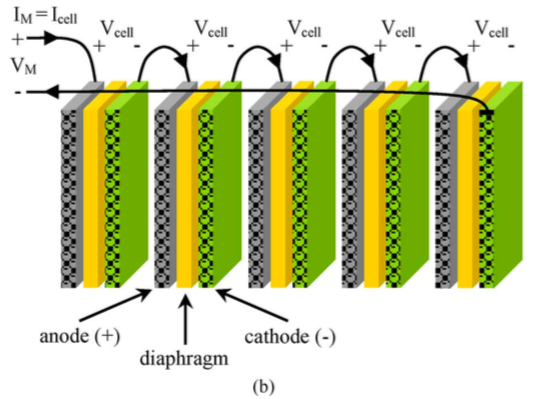
\includegraphics[width=7cm] {bipolar.png} 
\caption{Electrolyser configuration a)Monopolar configuration; b)Bipolar configuration.\cite{configuration}} 
\end{figure} 

\begin{table}
\begin{tabular}{|p{8cm}|p{8cm}|}
 \hline
 Unipolar & Bipolar \\ 
 \hline
 \multicolumn{2}{ | c |}{Advantages} \\

 \hline
 Simple design and therefore easy to fabricate & The compact structure reduces electrolyte ohmic loss, thus improves efficiency \\
 \hline
Do not have parasitic currents & Operate at higher temperature and pressure \\
 \hline
 Cells can be individually isolated and carry out maintenance & Operate at higher current density which increases rate of production\\
 \hline
 Low maintenance requiremnet & Small requirement in space\\
 \hline
  \multicolumn{2}{ | c |}{Disadvantages} \\
  \hline 
Large Ohmic losses due to high currents and low voltages &  Parasitic currents which cause efficiency loss and corrosion problems\\
   \hline 
Large space required & High requirements in precision and complex system design\\
\hline
 Large limitation in raising operating temperature and pressure & Production needs to be stopped for maintenance\\
 \hline
 Difficult to achieve small interelectrode gaps & Requirement for electrolyte circulation\\
 \hline
 Heavy intercell busbars & Requirement for external gas/electrolyte separator\\
 \hline
\end{tabular}
\caption{\label{tab:table-name}Pros and cons of monopolar and Bipolar configuration.\cite{configuration2} \cite{efficiency2} }
\end{table}
 
\subsubsection{Cell Geometry} 
Apart from adjusting the operating conditions, proper choice of cell geometry is another way to improve performance. Some of the key design parameters include size of inter-electrode gap, height and inclination of electrodes, and whether or not the separator is present. The smaller the gap between the electrodes, the smaller the volume of the electrolyte and thus the lower the ohmic overpotential. However, in the conventional configuration, reducing the inter-electrode gap could increase the contribution of cell resistance from gas bubbles, making the optimal gap to be larger than 2mm. This problem can be solved by adopting zero-gap configuration.\cite{zerogap}A series of experiments\cite{geometry} were conducted to identify the effects of electrode height and inclination, and it has been found that although selecting larger electrodes will enlarge the surface area and thus the current path, when the current density is large, higher efficiency can be achieved using smaller electrodes. This is 
because bubbles tend to accumulate at higher parts of the cell, increasing the void fraction. The experiments also showed that placing the electrodes at perfectly vertical position reduces the ohmic overpotential. The separator is another source of inefficiency, and these experiments showed that higher efficiency was found when the separator was absent. 

\subsubsubsection{Zero-gap Configuration}
The zero gap cell involves two porous electrodes that are compressed and in contact with the membrane, making the inter-electrode gap the same as the thickness of the membrane( $<$  0.5 mm).The bubbles are released from the rear of the electrodes, which also reduces the contribution of cell resistance from the gas bubbles. Between the porous electrode and the bipolar plate is the gas diffusion layer, which not only provides an electrical connection, but also allows the feed of the electrolyte and the release of oxygen and hydrogen.This configuration can be assembled by depositing a catalyst layer onto the electrode, and then compressed onto the membrane, and finally gaskets are assembled to avoid leaking.\cite{zerogap}The disadvantage of this configuration is the increased potential for the gas bubbles to block the electrode-membrane interface.
\begin{figure}[!htb]
   \begin{minipage}{0.48\textwidth}
     \centering
     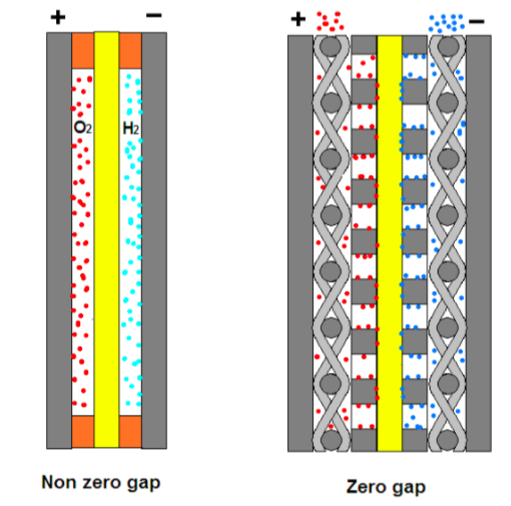
\includegraphics[width=.7\linewidth]{zerogap.png}
     \caption{Illustration of non-zero-gap and zer-gap configuration\cite{cathode2}}\label{Fig:Data1}
   \end{minipage}\hfill
   \begin {minipage}{0.48\textwidth}
     \centering
     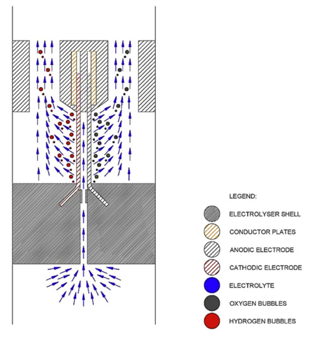
\includegraphics[width=.7\linewidth]{membraneless.png}
     \caption{Filtration mesh electrode housed in a rectangular single injection assembly.\cite{membraneless}}\label{Fig:Data2}
   \end{minipage}
\end{figure}

\subsubsubsection{Membrane-less Electrolyser}
In a conventional electrolyser, a membrane is used to separate the oxygen and hydrogen gases. However, membranes can be expensive to produce and may not be stable. Membraneless electrolysers have been developed to solve the problem. Figure 15 shows the principle of membraneless Divergent Electrode-Flow-Through (DEFT) alkaline electrolyser. The technology is based on the parallel arrangement of porous electrodes which are separated by an electrode gap.The liquid electrolyte is first introduced into the high pressure distribution chamber, and then the fluid is subsequently introduced into the gap between each electrode. Instead of using a membrane to separate the oxygen and hydrogen gases, the gases are separated by fluid mechanic forces.\cite{membraneless2} One of the biggest advantages of this design is that there are almost no gas bubbles forming between the electrodes, thus have the potential to operate at a higher current density than the conventional electrolyser. An appropriate electrolyte flow velocity is required to reduce the gas bubbles to a negligible volume, and also prevent gas contamination to ensure a high hydrogen purity. Using the membraneless DEFT technology, a hydrogen purity of 99.83\% can be achieved with an electrode gap of 2.5mm and a minimum velocity of 0.075m/s.



\subsubsection{Electrode Material} 
The anode material must have good conductivity, high catalytic activity, good mechanical stability, resistance to electrolyte corrosion, in addition to an acceptable cost. Currently, the mostly used anode is nickel or nickel based alloy. Nickel has good corrosion resistance compared with Stainless Steel or iron electrode and low price in alkaline medium. At the same time, nickel has high oxygen evolution potential and high oxygen evolution efficiency. One way to improve efficiency is to increase the electrode surface area in order to reduce the real current density and thus the activation overpotential. For example, a porous anode can be developed by sintering nickel powders, it has been shown that the porous high-surface area anodes have lower oxygen evolution overpotential than smooth anodes under elevated temperature and pressure (30bars, 200$^oC$). Sintered, porous nickel coating is an another way to reduce overpotential which involves a lower sintering temperature. It has also been shown that an increase in coating thickness will raise the exchange current density and reduce the overpotential. Comparable effects in overpotential reduction can be achieved by using Raney alloys such as Raney nickel, Raney cobalt or Raney nickel-cobalt which will be covered with Ni or Co oxides during electrolysis.\cite{anode} \cite{anode2}\\ \\
The cathode materials for hydrogen production in early age were mainly Pt, Pd and its alloys. Although these alloys have very low hydrogen evolution overpotential, they are expensive and can not be widely used to popularise.  So people put their eyes on cheap, low hydrogen overpotential alternatives such as Raney nickel or nickel based alloys like NiMo, NiSe and $NiS_2$. For cathode, the electrocatalyst's behaviours depend on its ability to adsorb hydrogen atoms, which is related to the strength of the metal hydrogen bond(M-H). A stronger M-H bond would reduce the HER activation energy. However, if the adsorption energy is too high, the desorption of hydrogen becomes difficult. Therefore, a suitable M-H bond strength is required for the cathode. It can be seen from figure 15 that Pt has the highest activity, and Ni also have suitable bond strength while being inexpensive at the same time. \cite{cathode2} Zhang compared the electrocatalytic activities of several nickel-based alloys(Ti/NiM where M represents different metals and Ni foil is the substrate). It can be shown from figure 16 that Ti/NiPt electrode has the highest catalytic activity, and they are all relatively stable. Ti/NiCo is the most suitable choice when electrolytic activity, stability and cost are all taking into account\cite{cathode}
\begin{figure}[H] 
\centering
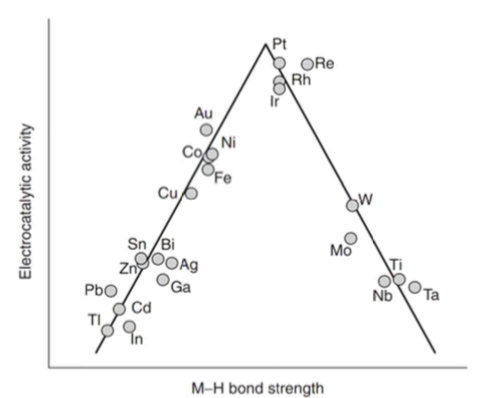
\includegraphics[width=6cm]{catalyst.png}
\caption{Electrocatalytic activity against M-H bond strengh\cite{cathode2}}
\end{figure}

\begin{figure}[H] 
\centering
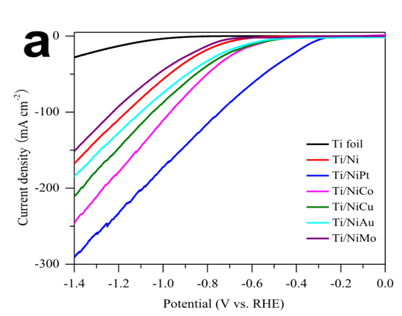
\includegraphics[width=6cm]{polarization.png}
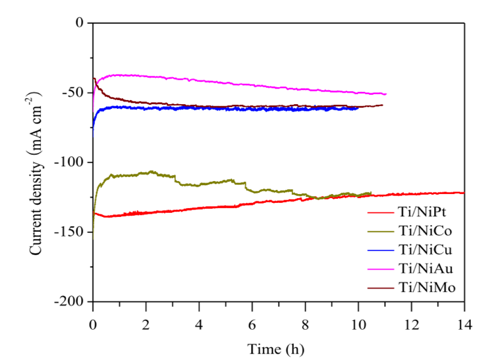
\includegraphics[width=6cm]{stability.png}
\caption{polarization curve for Ti/NiM electrode(left);Long term stability of catalytic Ti/NiM electrode for HER recorded at 1V(right) \cite{cathode}}
\end{figure}


\subsubsection{Electrolyte and Ionic Activator}
The selection criteria for the electrolyte include: high ionic conductivity;  does not decompose chemically under supplying voltage; lower volatility so is not removed with the product gas. Alkaline electrolyte is adopted instead of acid electrolyte because the corrosion problems is not as serious. KOH and NaOH solutions are common electrolyte choices and their conductivities at different temperatures are shown in figure 10. It is observable that KOH solution has higher specific conductivity than NaOH and is therefore used in this model. Although recirculation of electrolyte is designed, there will be some electrolyte loss in reality through gases(typically 1 mg KOH per $Nm^3$ H2). It is therefore necessary to adjust the amount of electrolyte in the cell. KOH is also cheaper than NaOH.

\begin{figure}[H]
\centering
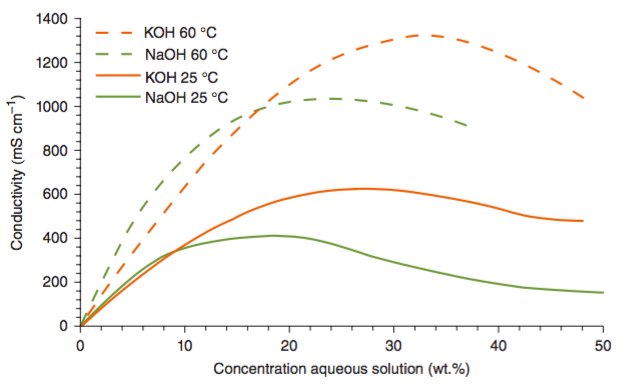
\includegraphics[width=8cm]{electrolytematerial.png}
\end{figure}
The energy consumption can be further reduced by the addition of an ionic activator. Lj et al. \cite{ionic}investigated the effect of adding an Novel ternary Ni $-$ Co $-$ Mo based ionic activator to the alkaline KOH solution. It has been found that the electrolyzer with in-situ activated electrolyte has an efficiency about 15\% higher than the standard KOH solution, and an energy consumption saving of about 17\%. The energy saving is proved to be more efficient at higher temperatures and current densities.During electrolysis, metal composites are electrodeposited in situ on cathode surface and exhibit better catalytic activity for hydrogen evolution reaction than those electro- deposited ex-situ. 

\subsubsection{Separator} 
The diaphragm(or microporous separators) , which is made of electrically insulating and hydrophilic materials, is used to separate the cathode and anode to prevent short circuit. The diaphragm also needs to be have high ionic conductivity for the hydroxide ions to pass through, while preventing the diffusion of hydrogen and oxygen gas bubbles, as well as unhindered intermixing of hydrogen saturated catholyte and oxygen saturated anolyte. Other requirements include low ohmic resistance and high resistance to corrosion in the alkaline environment. Asbestos membrane was used for a long time in the industry. However it has low resistance to corrosion and was forbidden because of its toxicity.A large number of inorganic and organic substitutes have been studied and currently Zirfon is the most widely used diaphragm. It contains the hydrophilic and inorganic $ZrO_2$ power and polysulfone network to increase the mechanical strength. The typically thickness of Zirfon diaphragm is 0.3mm, which is much thinner than the asbestos diaphragms. It also have a low ionic resistance(0.1-0.2$\Omega cm^2$)\cite{zirfon} In industry, the Zirfon diaphragm usually have a temperature limit of $120^oC$.\cite{pressure}\\\\
Ion exchange membrane can also be used as separator in water electrolysis, with the cation exchange membranes being more resistant than anion exchange membranes in alkaline environment and at elevated temperature. The cell is divided into two hydraulically separated compartments. The cation exchange membranes have negatively charged functional groups such as - SO3 or - COOH, and therefore only allows cations to pass through. \cite{ionexchange} The typical pores size is about $10^{-9}$ to1$ 0^{-8}$m.\cite{separator} Nafion perfluorosulfonate ion exchange membrane demonstrates promising performance. It has been shown that the performance can be improved by reducing the separator thickness, and increasing the operating temperature. One advantage of this type of separator is that it allows a very high operating temperature (220 - 250 $^oC$)\cite{separator3} before it loses stability. However, the biggest disadvantage is the high cost.\cite{separator2} 

\subsubsection{Ultrasound-aided Electrolysis}
Another way to enhance the energy efficiency is through coupling electrolysis with ultrasonic field. Li et al.\cite{ultrasound} investigated the effects of ultrasound on alkaline water electrolysis. The results showed that the cell voltage was lower in the presence of ultrasound,
especially at higher current density and lower electrolyte concentration. The experiment also indicated that the enhancement of the efficiency was generally greater at higher electrolyte concentration.The efficiency of Hydrogen production was increased in the range of 5 to18\% at higher current density under ultrasonic field and energy saving was up to 10 to 25\%. Other forms of external fields, such as magnetic field and super gravity field also have the effects of improving energy efficiency. The application of external field is useful because it accelerates the bubble detachment in the process. \cite{review}
%\begin{figure}[H]
%\centering
%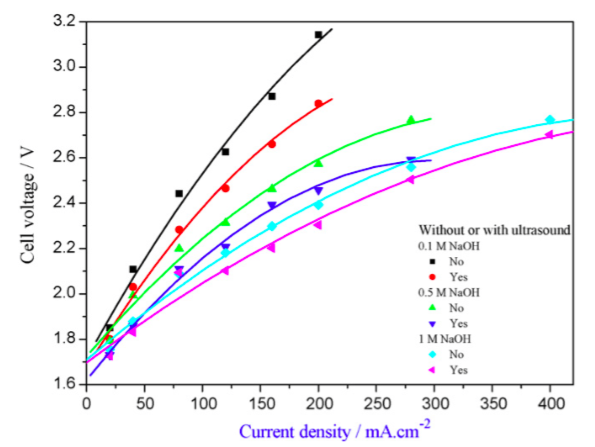
\includegraphics[width=8cm]{ultrasound.png}
%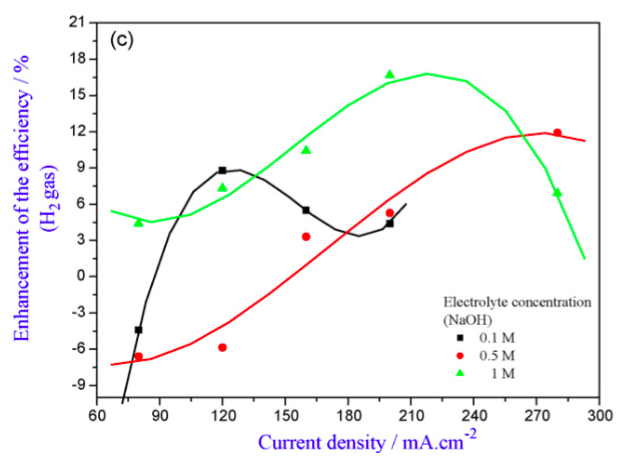
\includegraphics[width=8cm]{ultrasound2.png}
%\caption{Steady-state EI curves of alkaline water electrolysis with and without application of the ultrasonic field at different NaOH concentrations\cite{ultrasound}}
%\end{figure}



%\begin{figure}
%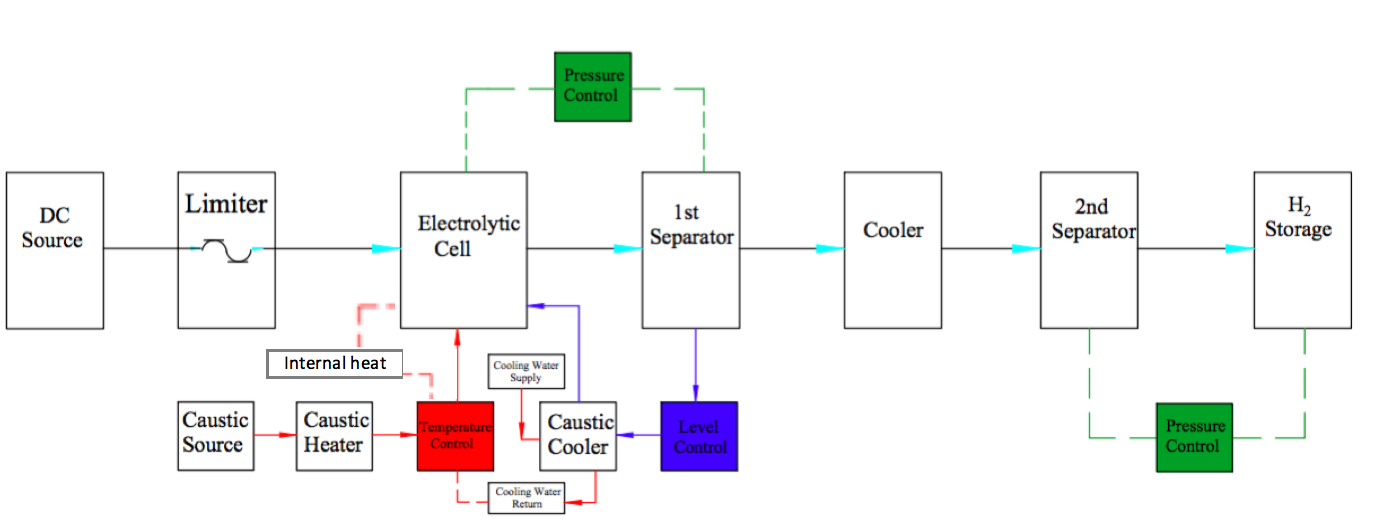
\includegraphics[width = 9cm]{control.png}
%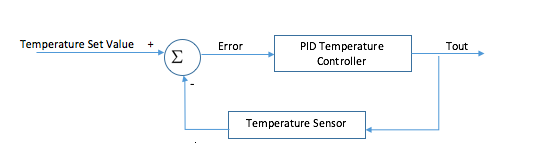
\includegraphics[width = 8cm]{PID.png}
%\caption{Electrolyzer control system}
%\end{figure}
\subsubsection{Stack Number}
The electrolyzer is designed so that the maximum hydrogen flow rate can be achieved(with a slight surplus) when all electrolysers are turned on and switched to their full capacity. The total power used in the electrolysis process can be calculated by,
%\begin{equation}
%P = N_{cell} V_{cell}  I_{cell} = N_{cell} V_{cell}  J_{cell} A
%\end{equation}
Assuming a typical cell area of 1$m^2$. The total number of cells required is 48970. Theoretically it is preferable to use a larger number of stacks with fewer cells in one stack, since this can reduce the power loss by reducing the minimum allowed input power. However,  the cost of a large amount of stacks could be quite high and they would also take up a large amount of space. Figure 15 shows the theoretical cumulative hydrogen production in January with different stack number. It can be seen that when the stack number is above 200, the hydrogen waste is less than 5\%. Therefore a stack number of 200(which could be divided into different electrolysers) and 245 cells per stack is an appropriate choice.
 \begin{figure}[H] 
 \centering
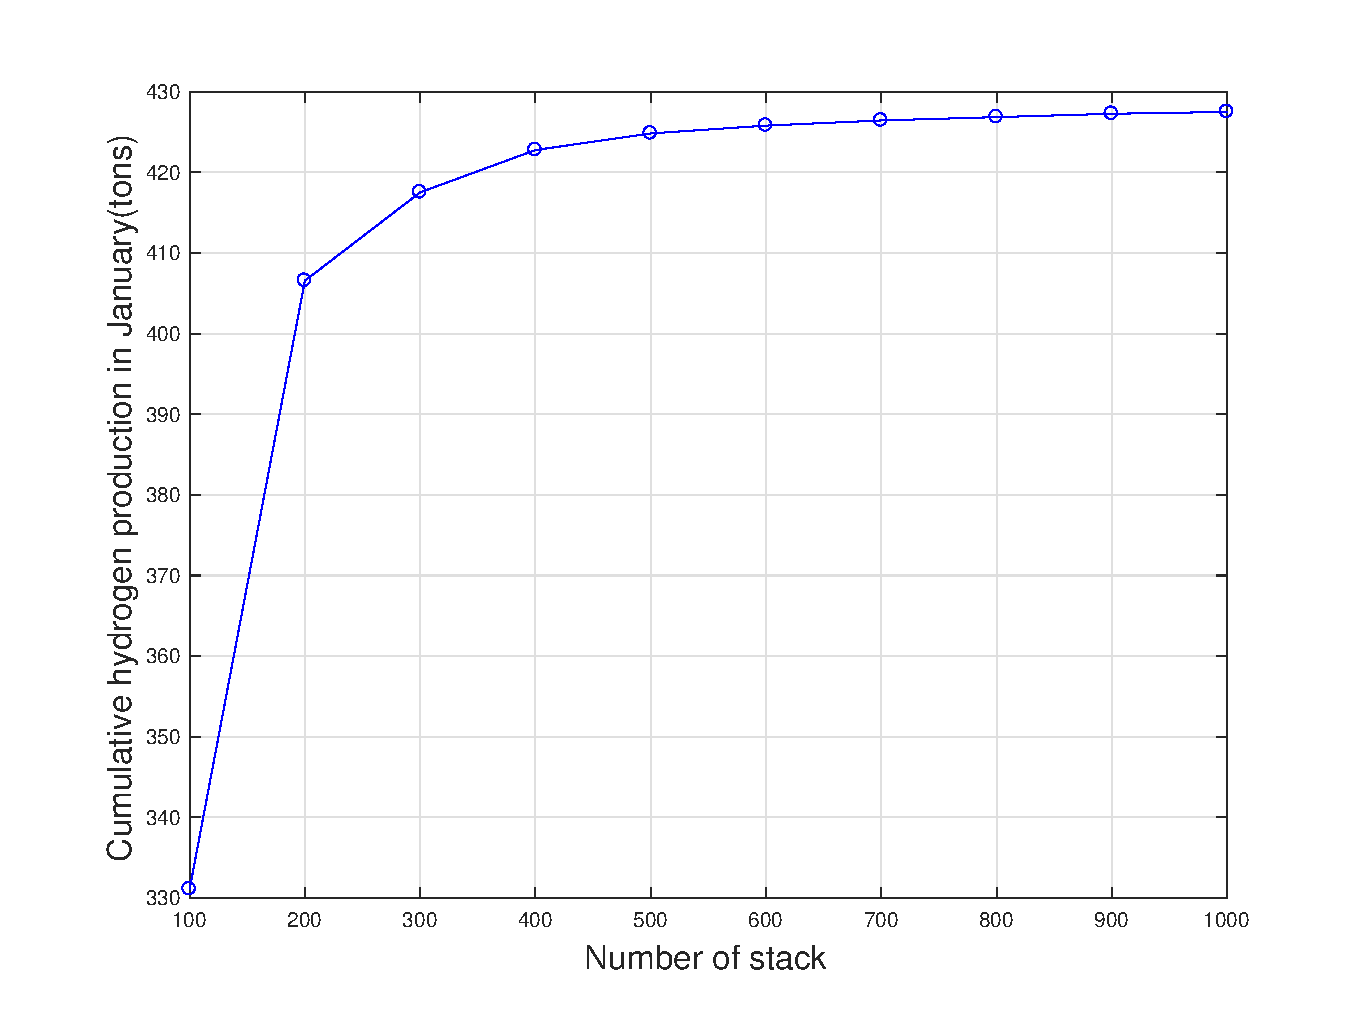
\includegraphics[width=7cm]{stack.eps}
\caption{Theoretical cumulative hydrogen production in January against number of stacks}
\end{figure}
 

\subsubsection{Thermal Model}
A lumped thermal capacitance model is established to determine the temperature of the electrolyte, which affects the V-I characteristics and system efficiency. The general energy balance can be represented by
\begin{equation}
C_t\frac{dT}{dt} = \dot{Q}_{gen}- \dot{Q}_{exch}-\dot{Q}_{cool}
\end{equation}
where 
\begin{equation}
\dot{Q}_{gen} = N_c(U-U_{tn})I 
\end{equation}
\begin{equation}
\dot{Q}_{exch} = \dot{n}_{H_2} C_p^{H_2}(T - Ta) + \dot{n}_{O_2}C_p^{O_2}(T - Ta)+ \dot{n}_{H_2O}C_p^{H_2O}(T - T_{in}^w)
\end{equation}
\begin{equation}
\dot{Q}_{cool} = \dot{m}_fC_p^f(T_o^f - T_{in}^f) 
\end{equation}
where $\dot{n}_i$ is the molar flow rates of product gases and water, $\dot{m}_f$ is the mass flow rate of the cooling water. $N_c$ is the number of cells in series and $C_p^f$ is the thermal capacity of fluid at constant pressure. At steady state, $\frac{dT}{dt} = 0$,  thus the required cooling water flow rate can be calculated, which is around 9 tons per hour for each stack.The above equations can also be used to predict the time required for the electrolyte to be heated up to the required temperature(assuming no heater to speed up the process), or used in temperature controller design which will be covered in the next session.

\subsubsection{Electrolyser Control System}
A control system needs to be installed in the electrolyser to keep it working properly. The CAD drawing at the start of this session included control logics such as temperature, pressure and level control.  A limiter is installed between the power source and electrolyser in order to prevent the low level power from passing through. The temperature control is designed to maintain the desired temperature. This can be achieved by controlling the flow rate of cooling water. Apart from the internal heat generated, a heater is also added as an additional heat source for better control. When the temperature is higher than the desired value, the cooling water flow rate increases to transfer heat more quickly.  Pressure is controlled to approximately 30 bar using pumps and pressure relief valves. Level controllers are installed in the electrolyser tank and gas-liquid separator to monitor the liquid level in the vessel to prevent leakage current and ensure that liquid in the separator is not carried to the next equipment. Due to space limit, only temperature control will be designed here. Closed loop PID control is the control mode most often associated with temperature controllers.\cite{control} To achieve better performance, a fuzzy pid model\cite{fuzzy} is adopted here. It is based on PID control algorithm and fuzzy control algorithm, which achieves fuzzy adjusting the PID parameters. The Simulink model shown in figure 14. 
\begin{figure}[H]
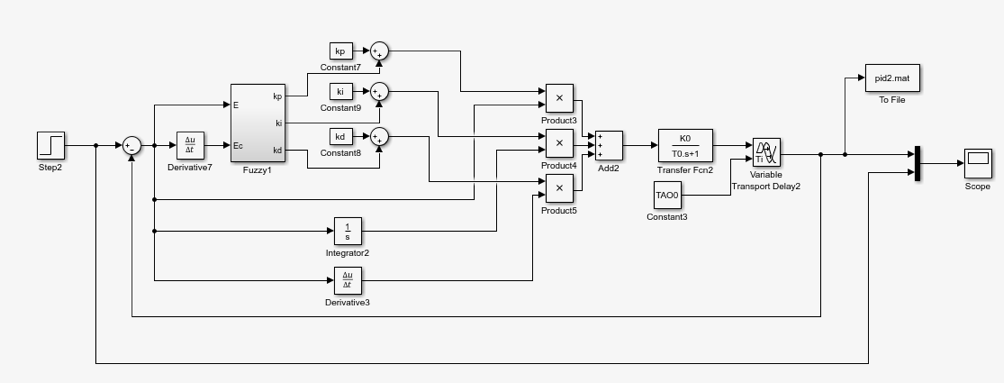
\includegraphics[with=10cm]{fuzzypid.png}
\caption{Fuzzy pid block diagram}
\end{figure}
The four equations in the thermal model session can be used to determine the transfer function, which is in the form of 
\begin{equation}
G(s) = \frac{K}{T_s\times s +1} 
\end{equation}
In reality, there should also be a time lag $e^{-\tau s}$ term in the temperature control system. 
The comparison between traditional pid controllers and fuzzy pid controllers are shown in figuire 15
\begin{figure}[H]
\centering
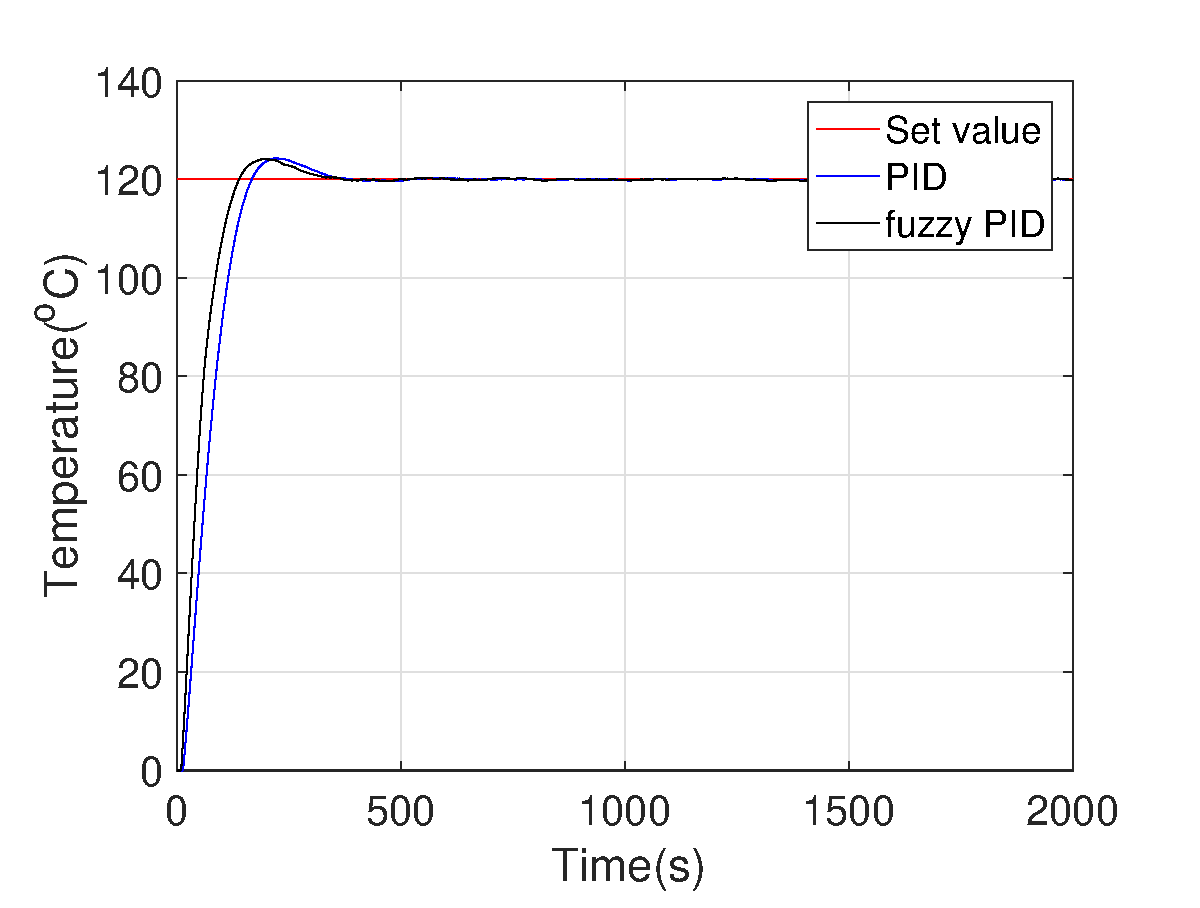
\includegraphics[width = 8cm]{pidpid.eps}
\caption{Comparison between pid and fuzzy pid controller under sensor noise}
\end{figure}
Both controllers have satisfactory performance with the fuzzy pid controller having faster response to changing temperature and smaller overshoot 



\subsubsection{Hydrogen  Storage }
The hydrogen storage system is required to supply the ammonia synthesis reactor with a constant hydrogen flow rate. There are three major ways to store the hydrogen gas produced , as compressed gas(above ground or underground), as a liquid or forming chemical bonding in solids(usually as metal hydrides).
When choosing a storage method, energy required, cost and safety are the major factors to consider and this is shown in table 3.
\begin{singlespace}
\begin{table}[H]
\begin{tabular}{ |p{4.2cm}|p{2.2cm}|p{2.5cm}|p{3.2cm}| p{2.7cm}|} 
 \hline
  & Compressed Gas(700bar) & Underground & Cryogenic Liquid   & Metal Hydride(NaAlH4) \\ 
 \hline
 Energy Required(MJ/kg) & 10.8  & 1.5  &43    & 15\\ 
 %\hline
 %Volumetric Energy Density(kWh/L) & 0.8 & 0 & 2.4 & 0.4\\
 \hline
Storage Cost(\$/kg) & 0.29  & 0.197  &1.48 & 0.116\\ 
 \hline
 Safety & High risk of fire or leak & Lower risk, potential leak due to cracks in rock & Risk of Overpressure & Zero Explosion Probability \\
 \hline
\end{tabular}
\caption{\label{tab:table-name}Operating conditions and key parameters.\cite{storage2}\cite{storage}\cite{gas2}\cite{gas3}}
\end{table}
\end{singlespace}

Storage as a compressed gas using the gas steel cylinders is the most simple and commercially mature storage method, and is therefore adopted in this model. Isothermal compression($\Delta T = 0$) is preferred as it requires minimum work input compared with isentropic compression, which is adiabatic. Several stages of compression is adopted to achieve the required compression ratio (a final pressure of 700-800bar with high strength materials) and the compressed gas needs to be cooled down after each stage.  The specific compression work can be calculated by \cite{gas}
\begin{equation}
w_i = RTZln(\frac{p2}{p1})
\end{equation}

where Z is the compressibility factor, and it is used here since the compressed gas is non-ideal. Z  is a function of temperature and pressure but is assumed to be constant here for simplicity. T is the temperature which is kept constant, $\frac{p2}{p1}$ is the compression ratio, where p1 is 30 bar. The compression work for different compression ratio is shown in figure 18. At a final pressure of 700bar, the compression work is 4.3 MJ/kg. In reality, the number should be higher than this since the process is not perfectly reversible or isothermal.(typical value is 10.8kJ/kg\cite{storage})

\begin{figure}[H]
\centering
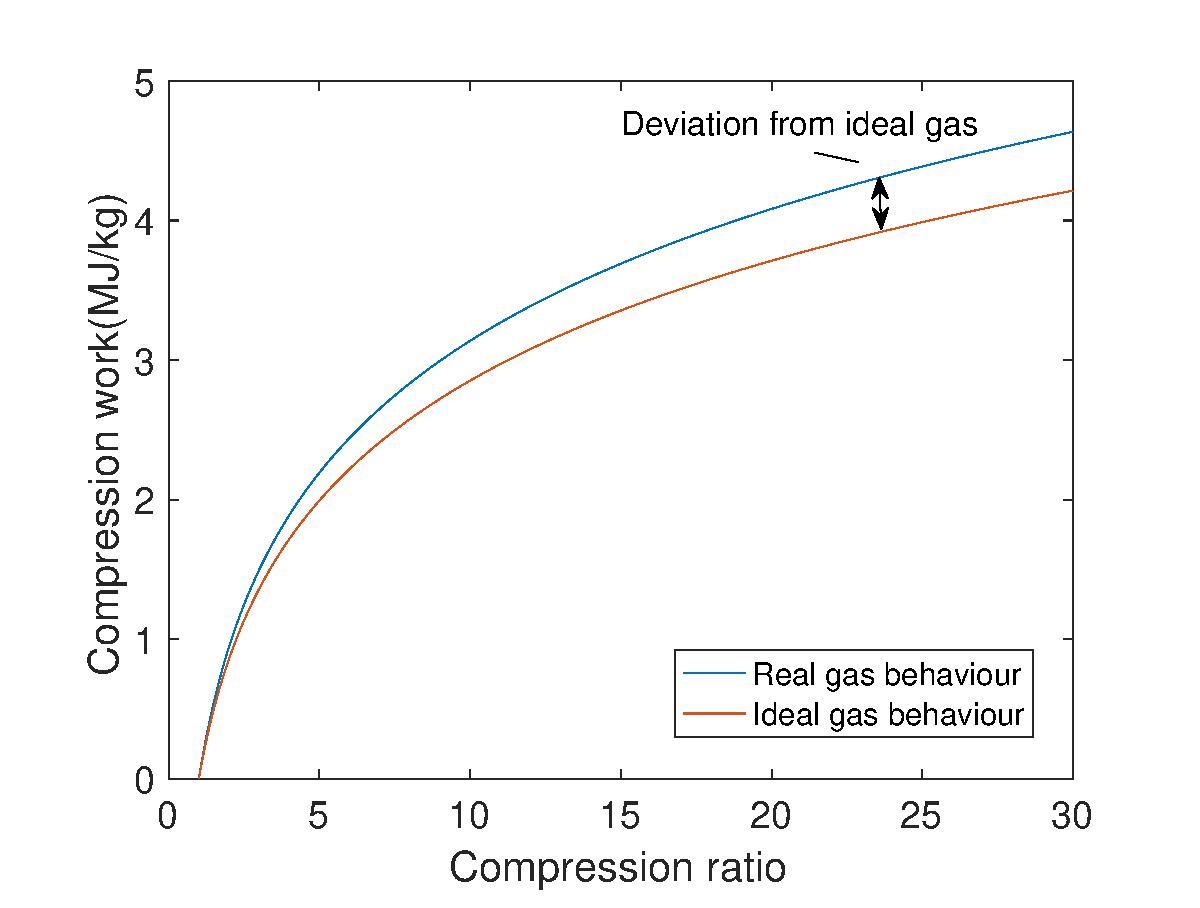
\includegraphics[width=7cm]{compression.eps}
\caption{Compression work as a function of compression ratio}
\end{figure}

Underground storage in salt cavern has been developed for compressed hydrogen gas.It has the benefits of increased storage capacity, low cost and safer operation. However, if the cavern is not already available, the cost of digging and reinforcing can be quite high, and the storage location is also restricted by geological factors.\cite{cons} Although liquid hydrogen has a higher energy density compared with compressed gas, liquifying hydrogen is rarely adopted as a storage method since a large amount of energy is required to achieve a very low temperature(-252$^oC$), it also needs fairly expensive heat-insulating materials. Metal hydrides is formed when a host metal is bonded with hydrogen atom to form a compound. When hydrogen needs to be recovered, the compound is supplied with heat to break the bonds. This method can significantly increase the energy density and also has lower risk compared with other storage methods. However, the cost of storage is quite high and strongly bonded hydrogen is hard to be recovered.\cite{storage3}


\subsection{System Simulation}
A system simulation is carried out based on power input profile,  demonstrating the results for 120 hours in November 2016.  Figure 16  shows the changes of  HHV efficiency and the ratio of power input and maximum input with time. As can be seen, the HHV efficiency is at a level of around 73\% for most of the time and increases when the power input is low. The gaps represent the time period when the power input is below the minimum allowed limit. Note that some power is lost during the AC to DC rectifier stage, the conversion efficiency is assumed to be 90\%. For simplification, the simulation assumed zero start-up time, zero response time and constant temperature at $120^oC$. Figure 17 demonstrates the cumulative production of hydrogen in this time period. Comparing this with the constant hydrogen consumption rate, the storage capacity requirement can be calculated. 
\begin{figure}[htb]
\centering
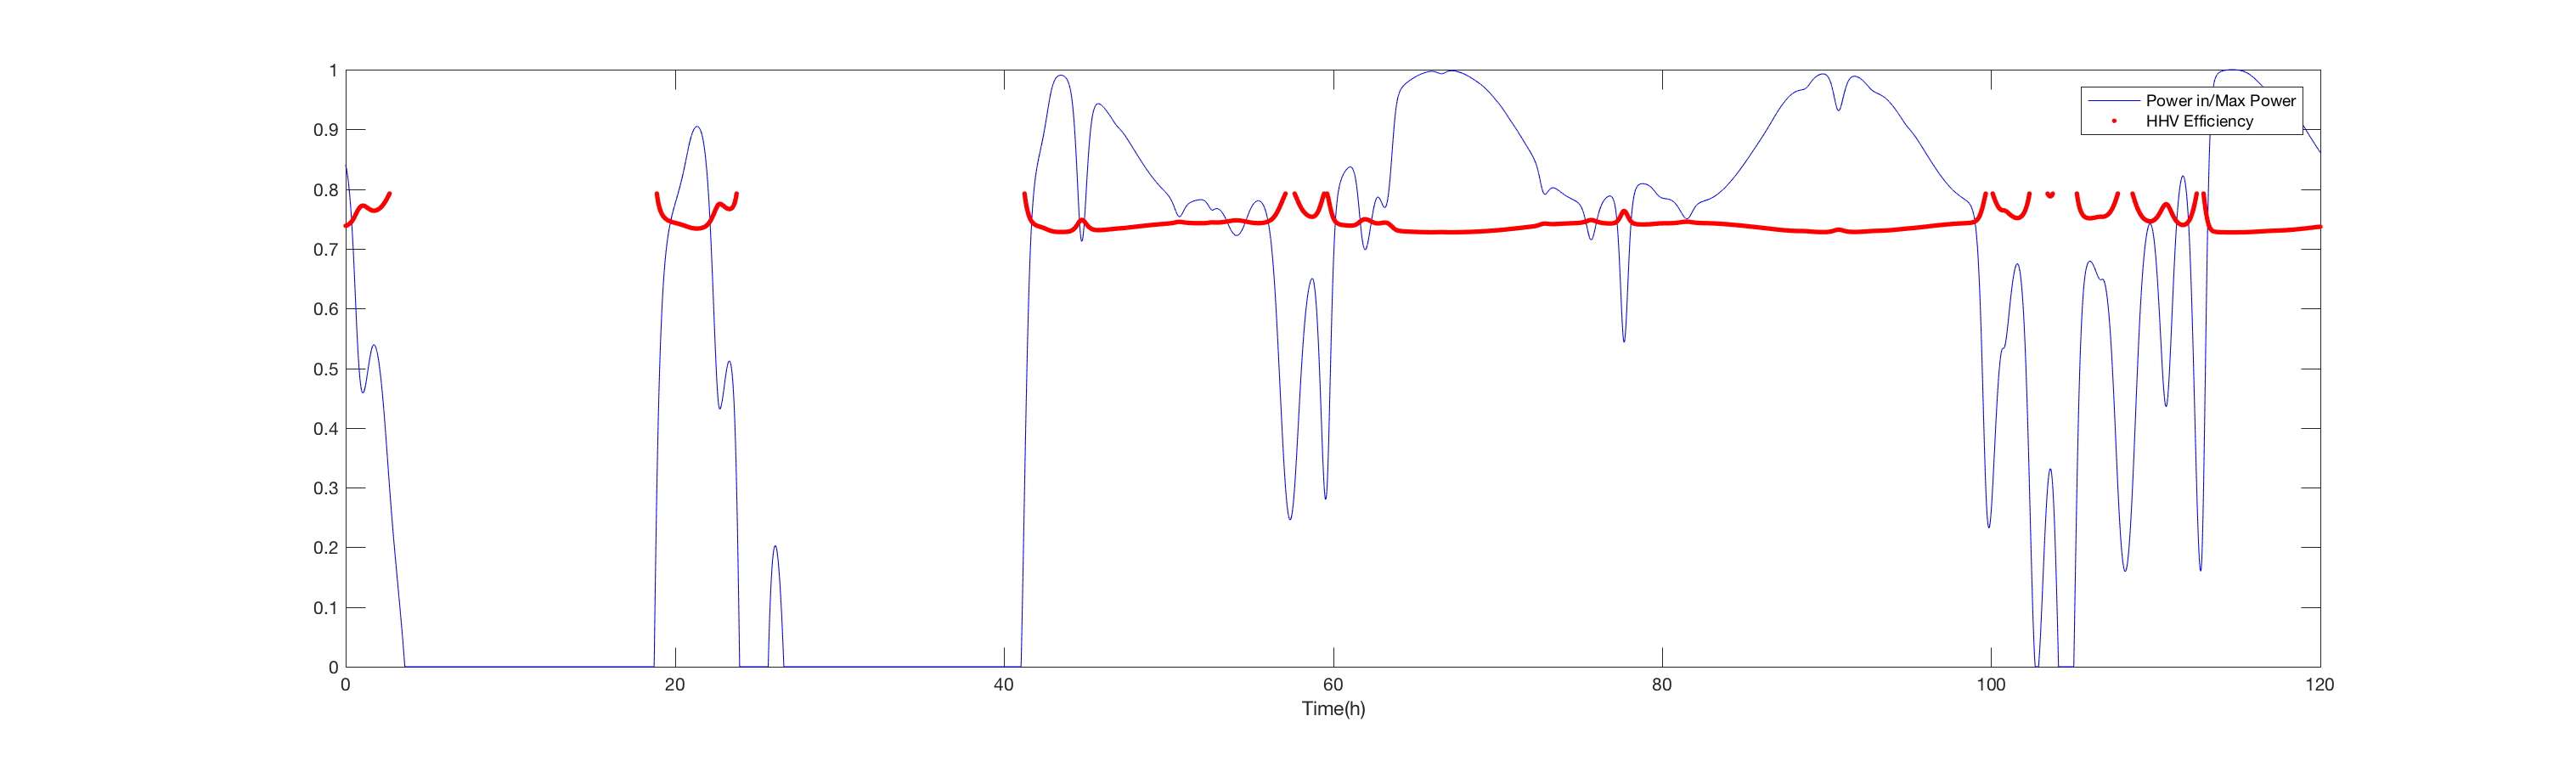
\includegraphics[width = 18cm]{simulation.eps}
\caption{HHV efficiency and Power/ Power max}
\end{figure}

\begin{figure}[htb]
\centering
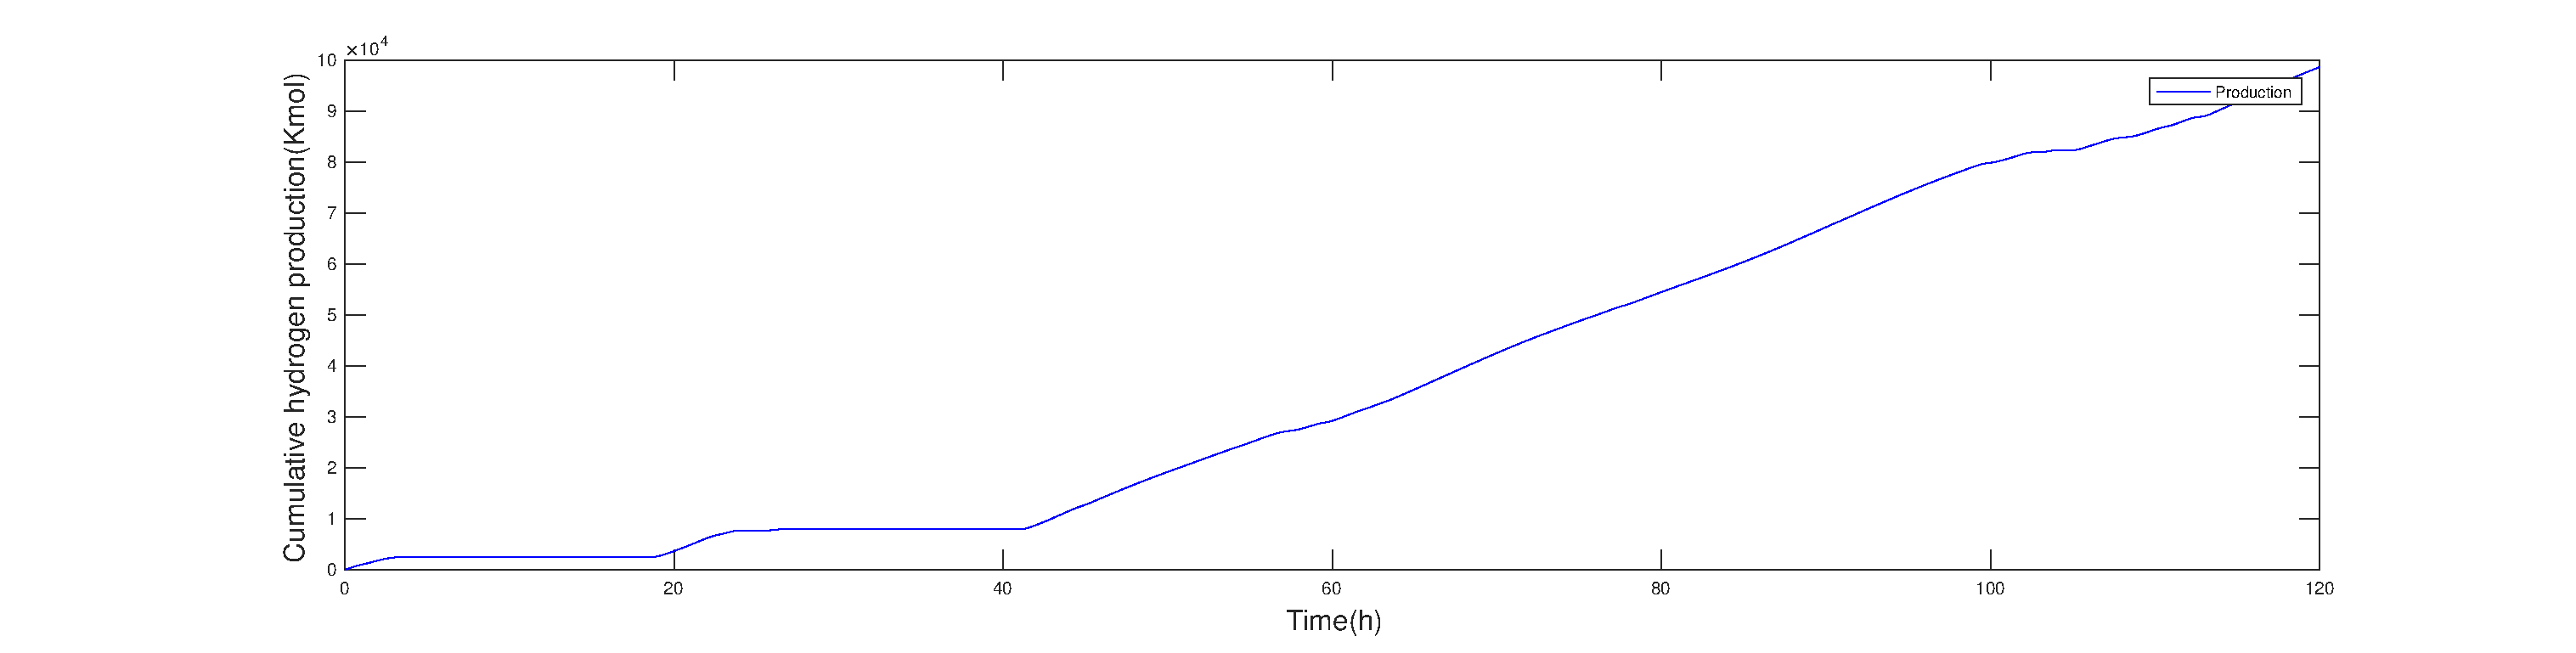
\includegraphics[width = 17cm]{cumulative.eps}
\caption{Cumulative production of hydrogen }
\end{figure}
\subsubsection{Costing}
\begin{singlespace}
\begin{longtable}{ |p{5.5cm}|p{2.5cm}|p{2.5cm}|p{2.9cm}|} 
%\begin{table}[H]
%\begin{tabular}{ |p{5.5cm}|p{2.5cm}|p{2.5cm}|p{2.9cm}|} 
 \hline
 \rowcolor{burntsienna}
  & Labour \$ & Material \$ & Total\$\\
  \hline
  \rowcolor{cyan}
   \multicolumn{4}{ | c |}{Direct Field Cost} \\
   \hline
  \rowcolor{LightCyan}
  \multicolumn{4}{ | c |}{Equipment Cost} \\
  \hline
  Vessels & 11350.74 & 113507.38 & 124858.12\\
  \hline
  Hydrogen Compressor & 22701.48 & 454029.51 & 476730.99\\
  \hline
  Drums/Filters & 4540.3  & 45402.95 & 49943.25\\
  \hline
  Cells & 56753.69 & 1225900 & 1282600 \\
  \hline
  Heat Exchangers & 4540.3 & 90805.9 & 95346.2\\
  \hline
  Pumps & 9080.59 & 181611.80 & 190692.4\\
  \hline
  %\rowcolor{cyan}
  \textbf{Subtotal Major Equipment} & \textbf{108967.08} & \textbf{2111237.23} & \textbf{2220204.31}\\
   \hline
    \rowcolor{LightCyan}
   \multicolumn{4}{ | c |}{Bulk Material Cost} \\
   \hline 
    \multicolumn{4}{ | c |}{\textbf{Civil/Structure/Architectural}} \\
   %Civil/Structure/Architectural  \\
   \hline 
   Foundations & & 28376.854  & 28376.84\\
   \hline
   Roads/Paving  & & 9080.59  & 9080.59\\
   \hline
   Building &  &113507.38  & 113507.38\\
   \hline
   Structural Steel & & 11350.74 & 11350.74\\
   \hline
    \multicolumn{4}{ | c |}{\textbf{Piping/Instruments}} \\
   \hline
   Pipe & 14755.96 & 34052.21 & 48808.17\\
   \hline
   Fittings & 9080.59 & 9080.59 & 18161.18\\
   \hline
   Valves & 11350.74 & 73779.80  & 85130.53\\
   \hline
   Cables & 13620.89 & 34052.21 & 47673.10\\
   \hline
   Instruments & 22701.48 &22701.48  & 45402.95\\
   \hline
   Control Valves & 17026.11 & 45402.95 & 62429.06\\
   \hline
    \multicolumn{4}{ | c |}{\textbf{Electrical}} \\
   \hline
   Cables &  13620.89  & 34052.21 & 47673.10\\
   \hline 
   DCS cabinet and card & 5675.37 & 4502.95 & 51078.32\\
   \hline
    \multicolumn{4}{ | c |}{\textbf{Paintings}} \\
   \hline
   Piping Painting & 5675.37 & & 5675.37\\
   \hline
   Equipment insulation & 9080.59 & & 9080.59\\
   \hline
   \multicolumn{4}{ | c |}{\textbf{Insulation}} \\
   \hline
   Piping Insulation & 17026.11 & & 17026.11\\
   \hline
   Equipment Insulation & 17026.11 & & 17026.11\\
   \hline
   \textbf{Subtotal Bulk Materials} & \textbf{303064.70} & \textbf{292849.04} & \textbf{595913.73}\\
   \hline

   \textbf{Total Direct Field Materials} & \textbf{412031.78} & \textbf{2404086.27} & \textbf{2816118.05}\\
   \hline
   \rowcolor{cyan}
 \multicolumn{4}{ | c |}{Indirect Field Cost} \\  
 \hline
 Construction management & 45402.95 & & 45402.95\\
 \hline
 Cranes & 56753.69 & & 56753.69\\
 \hline
 Scaffolding & 30646.99 & & 30646.99\\
 \hline
\textbf{Total Indirect Field Costs} & \textbf{132803.63} & & \textbf{132803.63}\\
 \hline
 \hline
 \rowcolor{cyan}
 \multicolumn{4}{ | c |}{Home Office/Miscellaneous} \\
 \hline
 Detailed Engineering & 31818.18 & & 31818.18 \\
 
 \hline
 
 
 Start-up & 12121.21 & & 12121.21\\
 \hline
\rowcolor{burntsienna}
 Total Costs Excluding UAP & 588774.81 & 2404086.27 &2992861.07\\
 \hline
 
Unallocated Provision  & & & 149643.05\\
\hline
\rowcolor{burntsienna}
Total Project Cost & & & 3142504.13\\
\hline
%\end{tabular}
\end{longtable}
\end{singlespace}

\subsubsection{Sustainability}
Alkaline electrolysis derived by renewable energies has a great potential to become a more vital hy- drogen production strategy due to its sustainable nature. Water is the only material input to the system and no greenhouse gases such as carbon dioxide will be produced in the process. While al- kaline electrolysis has a lower energy efficiency than the conventional hydrogen production methods such as natural gas reforming, the continuous advances in the electrolysis technologies could lower the production costs and make it more competitive and widely used in large scale projects.
\subsubsection{Safety}
The major risk in the electrolysis plant is the flammable mixture of oxygen and hydrogen gases.
Hydrogen has the NFPA 704's highest rating of 4 on the flammability scale. \cite{safety} This can happen if the gas crossover during the electrolysis is above the allowed limit, or if hydrogen is leaked to the air which is difficult to detect since its colourless, odourless, and tasteless. Hydrogen gas has a flammability range of 4-75\% in the air and it also has a very low ignition energy(as low as 17$\mu$J).To avoid this problem, 
before driving the hydrogen production equipment, it is necessary to fill the system with nitrogen until the oxygen content of the system is less than 1\%; Hydrogen leak alarm devices need to installed and electrolysis room should be set explosion-proof lights. Hydrogen flames are also nearly invisible, so flame detectors are needed. Also, all the equipment should be well grounded to prevent static electricity, which can cause hydrogen combustion and explosion. The leakage of the alkaline electrolyte is another potential risk. The HAZOP analysis is shown below.


{\fontsize{8pt}{7.5pt}\selectfont\tabcolsep=2.5pt\renewcommand\arraystretch{1.5}
\begin{longtable}{
|m{1.75cm}<{\centering}|m{3cm}<{\centering}|m{3cm}<{\centering}
|m{1.25cm}<{\centering}|m{1.1cm}<{\centering}
|m{3.5cm}<{\raggedright}|}
 \hline
 \rowcolor{cyan}
Deviation &Causes &Unmitigated Consequences &Likelihood &Risk Ranking &Recommendations\\
\hline
\multirow{11}*{More Flow} & {Hydrogen/oxygen control valve failure} &
{Cell reaction pressure drop, Electrolysis efficiency will be reduced} & Middle & Low & Add high flow alarm to response\\
\cline{2-7}
&{Cooling Water hand valves fully open by human error} &
No Hazard identified &&&\\
\cline{2-7}
&{Caustic control valve failed to fully open} &
{High level in cell, lead to overpressure, potential fatality} &
 Low & \multicolumn{1}{>{\columncolor{red}}c|}{High} &
{Add high level alarm to response; \par
Add high high level interlock to
trip reaction cell.}\\
\cline{2-7}
&{Feed water valve fully open by human error} &
{Flooding in the separator} &
 Low & Low & Add high level alarm to response;\\
\cline{2-7}
&{Nitrogen hand valve open by human error} &
Production unqualified. & Low &Low &
{Add blind flange between the two hand valves.}\\
\hline
\multirow{13}*{Less Flow}&
{Hydrogen/oxygen control valve failed fully close} &
{Overpressure lead to vessel/cell rupture potential fatality} &
 Low & \multicolumn{1}{>{\columncolor{red}}c|}{High} & {Add high Pressure alarm to response; \par
Add high high Pressure interlock
to trip reaction cell.}\\
\cline{2-7}
&{Cooling Water hand valves fully close by human error} & {Water carried with H2/O2, production unqualified} &  Low & Low& {Add high temperature alarm for the production to response}\\
\cline{2-7}
&{Caustic control valve failed fully closed} & {Low level in cell, lead to reaction stop} &  Low &Low &Add Low level alarm to response.\\
\cline{2-7}
&{Feed water valve fully closed by human error} & {Low level in cell, lead to reaction stop} &  Low & Low & Add Low level alarm to response.\\
\hhline{~|------}
&Pump Failure &
{Backflow of gases, causing flammable gas mixture} &  Low & \multicolumn{1}{>{\columncolor{red}}c|}{High} & Use valves to prevent gas backflow\\
\hhline{~|------}
&Facility Leakage & {Hydrogen leak into facilities, risk of explosion} &  Low & \multicolumn{1}{>{\columncolor{red}}c|}{High} & { Install hydrogen sensor and leak alarm for emergency shut down}\\
\hhline{~|------}
&Valve or pipe blockage & Bursting of pipes &Low &\multicolumn{1}{>{\columncolor{red}}c|}{High} &Install blockage detectors\\
\hhline{~|------}
&Water level too low & Leakage current & Low &\multicolumn{1}{>{\columncolor{red}}c|}{High} &Check the level controller\\
\hline
No flow &\multicolumn{6}{c|}{Refer to less flow}\\
\hline
\multirow{4}*{Reverse Flow}& {Caustic source shut down due to unkown reason} & {Hydrogen reverse to caustic system, cause jet fire if leaked, potential people injury} & Safety & Low & Middle & Add check valve.\\
\cline{2-7}
&{Feed water source shut down due to unkown reason} & {Hydrogen reverse to feed water system, cause jet fire if leaked, potential people injury} & Low & Low & Add check valve.\\
\hline
High Pressure & {Pressure control system fails; Blockage; Pump failures} & {Facilities breakdown, potential explosion; low gas purity} &  Low & \multicolumn{1}{>{\columncolor{red}}c|}{High} &
Pressure sensor installed for
emergency shutdown\\
\hline
Low Pressure& Pump fails; pressure controls fails; leak in reactor& Electrolyte boils if operating above 100$^\circ$C; more work at hydrogen storage stage &  Low & Middle &
Check the pumps; \par
Check for any leakage\\
\hline
High Temperature & Cooling water flow rate too low; Heat exchanger malfunction&
Material corrosion and mechanical failure such as membrane rupture;
Electrolyte boiling& Low &\multicolumn{1}{>{\columncolor{red}}c|}{High}&
Check the cooling water
valves \par
Check temperature controller\\
\hline
Low Temperature & Cooling water flow rate too high; Heat exchanger malfunction& Low efficiency &Low &Low &
Check the cooling water valves \par
Check temperature controller\\
\hline
Rupture/ Leak &Tube rupture in cooler& High pressure cooling water, could cause jet fire if leaked& Low &Middle &Add pressure relieve valves\\
\hline
Contaminants/ Composition& Water deionization stage
malfunction&
Side reactions; reduce lifetime &Low &Middle& Add anaylser for feed water quality\\
\hline
Chemical Hazards& Electrolyte concentration too high& Cell or pipeline leakage;corrosion of membrane and electrodes& Low &\multicolumn{1}{>{\columncolor{red}}c|}{High}&
Upgrade materials. \par
Check recirculation pump \par
Install PH meter linked to alarms\\
\hline
\end{longtable} }
%
\includepdf[pages=2,angle=180]{hazop.pdf}
%
\includepdf[pages=3,angle=180]{hazop.pdf}




\subsection{Conclusion} 
Alkaline electrolysis integrated with wind energy to produce hydrogen is a mature technology with a great potential to reach a larger production scale. 
This chapter reviewed the thermodynamics and kinetic analysis of the electrolysis system, as well as several sources of inefficiency. It was found that choosing optimum operating conditions such as elevated temperature and pressure, proper cell geometry and material selections are the key to improve system performance. 

......Justify costing data sources;finish sustainability,Enlarge some images that are currently small; fix merge errors;explain control part in more details; Write more on conclusion part....

\singlespacing
%\linespread{0.4}
\begin{thebibliography}{99}
\linespread{1} 
\bibitem{purity}
V. L. KuchaevE. N. ShapatinaA. K. Avetisov, Mechanism of oxygen poisoning of ammonia synthesis catalyst
\bibitem{gas}
Hydrogen Science and Engineering, Materials, Processes, Systems and Technology, Wiley-VCH
\bibitem{gas2}
Zehra Yumurtac? and Nur Bekiroglu, Yildiz Technical University Mechanical Engineering Faculty, TR 34349, Besiktas Istanbul, ECONOMICAL ANALYSIS OF GASEOUS AND LIQUID HYDROGEN STORAGE AND TRANSPORTATION
\bibitem{gas3}
L. Kit Heung, L. Kit Heung, Savannah River Technology Center Aiken, SC 29808 USAUsing Metal Hydride to Store Hydrogen
\bibitem{specification}
Study on development of water electrolysis in the EU Fuel Cells and Hydrogen Joint Undertaking
\bibitem{cons}
Above Ground Vs. Underground Storage Tanks: Pros and Cons,http://www.communicationsetc.net/above\-ground\-vs\-underground\-storage\-tanks\-pros\-and\-cons/
\bibitem{rate} 
Alhassan Salami Tijania, Nur Afiqah Binti Yusupb, A. H. Abdol Rahimc
%\textit{The \LaTeX\ Companion}. 
Mathematical modelling and simulation analysis of advanced alkaline electrolyzer system for hydrogen production
\bibitem{gibbs} 
Joonas Koponen,Review of water electrolysis technologies and design of renewable hydrogen production systems
\bibitem{thermoneutral}
Allebrod, Frank; Mogensen, Mogens Bjerg; Hjelm, Johan; Ebbesen, Sune Dalgaard, High Temperature and Pressure Alkaline Electrolysis
\bibitem{reversible}
M. Hammoudi, C. Henao, K. Agbossou, Y. Dube?, M.L. Doumbia, New multi-physics approach for modelling and design of alkaline electrolyzers
\bibitem{conductivity}
R.J. Gilliama,, J.W. Graydonb, D.W. Kirkb, S.J. Thorpea, A review of specific conductivities of potassium hydroxide solutions for various concentrations and temperatures
\bibitem{activation}
Richard L. Doyle and Michael E.G. Lyons, The Oxygen Evolution Reaction: Mechanistic Concepts and Catalyst Design
\bibitem{activation1}
Milewski, J, Guandalini, G  Campanari, S 2014, Modeling an alkaline electrolysis cell through reduced-order and loss-estimate approaches?, Journal of Power Sources, vol. 269, pp. 203?211.
\bibitem{activation2}
Hammoudi, M, Henao, C, Agbossou, K, Dub�, Y, Doumbia, M 2012, New multi- physics approach for modelling and design of alkaline electrolyzers?, International Journal of Hydrogen Energy, vol. 37, no. 19, pp. 1389513913.
\bibitem{activation3}
H. Wendt and V. Plzak. Electrocatalytic and thermal activation of anodic oxygen- and cathodic hydrogen-evolution in alkaline water electrolysis. Electrochimica Acta, 28(1):27?34, 1983.
\bibitem{activation4}
Christian Henao, Kodjo Agbossou, Mhamed Hammoudi, Yves Dub�, Alben Cardenas, Simulation tool based on a physics model and an electrical analogy for an alkaline electrolyser
\bibitem{efficiency}
RodneyL. LeRoy*andChristopherT. Bowen, The Thermodynamicsof AqueousWater Electrolysis
\bibitem{efficiency2}
Alfredo Ursua, Member IEEE, Luis M. Gand, and Pablo Sanchis, Member IEEE, Hydrogen Production From
Water Electrolysis: Current Status and Future Trends
\bibitem{geometry}
N. Nagai, M. Takeuchi,T. Kimura, T. Oka, Existence of optimum space between electrodes on hydrogen production by water electrolysis
\bibitem{zerogap}
A.Ursua.Hydrogen Production From Water Electrolysis: Current Status and Future Trends Proceedings of the IEEE�100(2):410-426���February 2012
\bibitem{bubble}
H.Vogt, The actual current density of gas-evolving electrodes Notes on the bubble coverage
\bibitem{bubble2}
H.Vogt, R,J, Balzer, The bubble coverage of gas-evolving electrodes in stagnant electrolytes
\bibitem{void}
Kitipong Tangphanta, Kaokanya Sudapraserta, z, and Suthin Channarong,Mathematical Modeling of Electrical Conductivity
in Electrolyte Solution between Two Gas Evolving Electrodes
\bibitem{void2}
Bhanu kiran.A1, Y.V.Ramana murty, Mathematical Modelling and Simulation Analysis of Alkaline Water Electrolyser for Stationary Electrolyte in Atmospheric Pressure
\bibitem{currentdensity}
Kai Zeng 1, Dongke Zhang,Recent progress in alkaline water electrolysis for hydrogen production and applications
\bibitem{currentdensity2}
Ugljesa Babic, Michel Suermann, Felix N. B�chi, Lorenz Gubler, Thomas J. Schmidt, Critical Review?Identifying Critical Gaps for Polymer Electrolyte Water Electrolysis Development
\bibitem{temp}
R. L. LERoY*, INDUSTRIAL WATER ELECTROLYSIS: PRESENT AND FUTURE
\bibitem{pressure}
Nicolas Guillet and Pierre Millet, Alkaline Water Electrolysis
\bibitem{pressure2}
Joonas Koponen, Review of water electrolysis technologies and design of renewable hydrogen production systems

\bibitem{configuration}
A. Ursua, BHydrogen production with alkaline electrolyzers: Electrochemical modelling, electric power supplies
and integration with renewable energies,[ (in Spanish) Ph.D. dissertation, Dept. Electr.
\bibitem{zerogap}
Robert Phillips,a and Charles W. Dunnill,  Zero Gap Alkaline Electrolysis Cell Designs for
 Renewable Energy Storage as Hydrogen Gas
\bibitem{membraneless}
M.I. Gillespiea, R.J. Kriek, Hydrogen production from a rectangular horizontal filter press Divergent Electrode-Flow-Through (DEFTTM) alkaline electrolysis stack
\bibitem{membraneless2}
M.I. Gillespie, F. van der Merwe, R.J. Kriek, Performance evaluation of a mem-
braneless divergent electrode-flow-through (DEFT) alkaline electrolyser based on optimisation of electrolytic flow and electrode gap, J. Power Sources 293 (2015) 228?235.

\bibitem{configuration2}
Tilak, B, Lu, P, Colman, J,  Srinivasan, S 1981, Chapter 1  Electrolytic production of hydrogen, in: Bockris, J, Conway, B, Yeager, E \& White, R, Comprehensive treatise of electrochemistry, volume 2: Electrochemical processing, Plenum Press, New York.
\bibitem{ionic}
Ivana M.PerovicPetar Z.LausevicGvozden S.TasicBojan B.RadakVladimir M.Nikolic,Sladjana Lj.MaslovaraMilica P.Marceta Kaninsk, Novel ternary Ni?Co?Mo based ionic activator for efficient alkaline water electrolysis
\bibitem{anode}
D. E. Hall, Electrodes for Alkaline Water Electrolysis, Inco Research \& Development Center, Incorporated, Sterling Forest, Suern, New York 10901
\bibitem{anode2}
D. E. Hall, Alkaline Water Electrolysis Anode Materials, American Cyanamid Company, Chemical Research Laboratories, Stamford, Connecticut 06904
\bibitem{cathode}
High-efficiency and stable alloyed nickel based electrodes for hydrogen evolution by seawater splitting, Zhang,Li,Yang,Fa,Ge. Journal of Alloys and Compounds.732 (2018) 248-256
\bibitem{cathode2}
Kjartansd�ttir, Cecil�a Krist�n; Moller, Per, Development of Hydrogen Electrodes for Alkaline Water Electrolysis
\bibitem{zirfon}
Ph. VERMEIREN, W. ADRIANSENS, J. P. MOREELS and R. LEYSEN,  EVALUATION OF THE ZIRFONj SEPARATOR FOR USE IN ALKALINE WATER ELECTROLYSIS AND Ni-H, BATTERIES
\bibitem{separator}
Diogo M. F. SantosI,; C�sar A. C. SequeiraI; Jose L. Figueiredo, Hydrogen production by alkaline water electrolysis
\bibitem{ionexchange}
Hanna Jaroszek, Piotr Dydo, Ion-exchange membranes in chemical synthesis ? a review
\bibitem{separator2}
Karel Vazac, Martin Paidar, Martin Roubal�k, Karel Bouzek, Impact of the Cation Exchange Membrane Thickness on the Alkaline Water Electrolysis
\bibitem{separator3}
YEO, S. C.  EISENBERG, A. 1977. Physical Properties and Supermolecular Structure of Perfluorinated
Ion-Containing (Nafion) Polymers. Journal of Applied Polymer Science, 21, 875-898.
\bibitem{ultrasound}
Sheng-De Li, Cheng-Chien Wang, Chuh-Yung Chen,Zhancheng Guo, Water electrolysis in the presence of an ultrasonic field
\bibitem{review}
Mingyong Wang,Zhi Wang,Xuzhong Gong ,The intensification technologies to water electrolysis for hydrogen production ? A review

\bibitem{control}
Appendix F:PID Temperature Control https://www.lakeshore.com/Documents/LSTC\_appendixF\_l.pdf
\bibitem{fuzzy}
WANG Haiqing, JI Changying, LIU Tongzhao, GAO Feng, XIAN Jieyu, Modeling and Simulation ofFuzzy Self-tuning PID Temperature Control System




\bibitem{storage}
Monterey Gardiner, Energy requirements for hydrogen gas compression and liquefaction as related to vehicle storage needs, https://www.hydrogen.energy.gov/pdfs/9013\_energy\_requirements\_for\_hydrogen\_gas\_compression.pdf
\bibitem{storage2}
L. Kit Heung Savannah River Technology Center Aiken, SC 29808 USA, Using Metal Hydride to Store Hydrogen, https://pdfs.semanticscholar.org/b781/192e2624db103d1b615502dd44354eff9b52.pdf
\bibitem{storage3}
Wade A. Amos, National Renewable Energy Laboratory, Costs of Storing and Transporting Hydrogen


\bibitem{safety}
https://en.wikipedia.org/wiki/Hydrogen\_safety



\end{thebibliography}










%\end{document}






